\RequirePackage{fix-cm}
\RequirePackage{amsmath} % solve problem with redefining \vec
%
%\documentclass{svjour3}                     % onecolumn (standard format)
%\documentclass[smallcondensed]{svjour3}     % onecolumn (ditto)
%\documentclass[smallextended]{svjour3}       % onecolumn (second format)
%\documentclass[twocolumn]{svjour3}          % twocolumn
%

%\documentclass[smallextended, draft]{svjour3}
\documentclass[smallextended]{svjour3}

% double spacing required for MGS submission
\usepackage{setspace}
\doublespacing

\smartqed  % flush right qed marks, e.g. at end of proof
%
\usepackage{graphicx}
% \usepackage{amsmath}
\usepackage{mathptmx}      % use Times fonts if available on your TeX system
\usepackage[misc]{ifsym}

\usepackage{xcolor}
\usepackage{url}
\usepackage{hyperref}
\makeatletter
\renewcommand*{\eqref}[1]{%
  \hyperref[{#1}]{\textup{\tagform@{\ref*{#1}}}}%
}
\makeatother

% \usepackage{mathptmx}      % use Times fonts if available on your TeX system
%
% insert here the call for the packages your document requires
%\usepackage{latexsym}
% etc.

%%%%%%%%%%%%%%%%%% my personal header %%%%%%%%%%%%%%%%%%%
% \usepackage{natbib} % for \citet and \citep
% \setcitestyle{aysep={}}
\usepackage[authoryear]{natbib}
\bibpunct{(}{)}{}{a}{}{;}
\newcommand{\doi}[1]{doi: \href{http://dx.doi.org/#1}{#1}}

\usepackage{lineno}
\linenumbers

% \usepackage{makecell} % for multiple lines withinin one cell
% \usepackage{booktabs} % for more space between rows in a table
% \usepackage[flushleft]{threeparttable} % for also including table notes

% \usepackage{sidecap}
\usepackage{hyperref}
% \usepackage[labelfont=bf]{caption}
\usepackage{amsfonts}
\usepackage{amssymb}


\usepackage{enumerate}
%\usepackage{bm} % for bold vectors \bm{v}
\usepackage{bbm} % indicator function \mathbbm{1}
%\usepackage{pdflscape} % landscape
%\usepackage[flushleft]{threeparttable}
%\usepackage{booktabs} % for \toprule

\spnewtheorem{mytheorem}{Theorem}{\bf}{\rm}
\spnewtheorem{myproposition}{Proposition}{\bf}{\rm}
\spnewtheorem{mylemma}{Lemma}{\bf}{\rm}
\spnewtheorem{myremark}{Remark}{\bf}{\rm}

% \usepackage{chngcntr}
\usepackage{apptools}
\AtAppendix{\counterwithin{mytheorem}{section}}
\AtAppendix{\counterwithin{myproposition}{section}}
\AtAppendix{\counterwithin{definition}{section}}
\AtAppendix{\counterwithin{mylemma}{section}}
\AtAppendix{\counterwithin{myremark}{section}}
% \AtAppendix{\setcounter{equation}{0}}
\AtAppendix{\counterwithin*{equation}{section}}
\AtAppendix{\renewcommand{\theequation}{\thesection.\arabic{equation}}}

% matrices and vectors
\renewcommand{\tens}[1]{\mathrm{#1}}
\renewcommand{\vec}[1]{\mathbf{#1}}

% treatment of units
\usepackage{siunitx}
\DeclareSIUnit\year{yr}
\DeclareSIUnit\carbon{C}

% real numbers, natural numbers, probability measure, expected value
\newcommand{\R}{\mathbb{R}}
\newcommand{\N}{\mathbb{N}}
\renewcommand{\P}{\mathbb{P}}
\newcommand{\E}{\mathbb{E}}
\newcommand{\TT}{\mathcal{T}}
% entropy
\renewcommand{\H}{\mathbb{H}}

% probability distributions
\newcommand{\PH}{\operatorname{PH}}
\newcommand{\Exp}{\operatorname{Exp}}
\newcommand{\Poi}{\operatorname{Poi}}

% put limits under sum, int, lim
\newcommand{\suml}{\sum\limits}
\newcommand{\prodl}{\prod\limits}
\newcommand{\intl}{\int\limits}
\newcommand{\liml}{\lim\limits}

% d/dt not italic
\newcommand{\deriv}[1]{\frac{\operatorname{d}}{\operatorname{d}#1}}
\newcommand{\dd}[1]{\,\mathrm{d}#1}
\newcommand{\pderiv}[1]{\frac{\partial}{\partial #1}}

% units
\newcommand{\peta}{\mathrm{P}}
\newcommand{\gC}{\mathrm{gC}}
\newcommand{\yr}{\mathrm{yr}}
\newcommand{\meter}{\mathrm{m}}
\newcommand{\bits}{\mathrm{bits}}
\newcommand{\nats}{\mathrm{nats}}

% other commands
\newcommand{\vnorms}[1]{\|#1\|}
\newcommand{\transpose}{T}
\newcommand{\diag}{\operatorname{diag}}
% \newcommand{\ie}{i.e.}
\newcommand{\ie}{that is}
% \newcommand{\eg}{e.g.}
\newcommand{\eg}{for example}

% words
\newcommand{\pdf}{probability density function}
\newcommand{\NPP}{\ensuremath{\mathrm{NPP}}}

%% pure editing commands
\newcommand{\red}[1]{\textcolor{red}{#1}}

% avoid italics for definitions, use `` '' instead
\renewcommand{\emph}[1]{``#1''}


%%%%%%%%%%%%%%%%%% end of my personal header %%%%%%%%%%%%%%%


% Insert the name of "your journal" with
\journalname{Mathematical Geosciences}
%

\begin{document}

\title{Information content and maximum entropy of compartmental systems in equilibrium%\thanks{Grants or other notes
%about the article that should go on the front page should be
%placed here. General acknowledgments should be placed at the end of the article.}
}
%\subtitle{Transit time and system age densities for linear autonomous compartmental models}

\titlerunning{Entropy in compartmental models}        % if too long for running head

\author{Holger Metzler \and Carlos A. Sierra}

%\authorrunning{Short form of author list} % if too long for running head

\institute{Holger Metzler \at
  Max Planck Institute for Biogeochemistry,
  Hans-Kn\"oll-Str. 10,
  07745 Jena,
  Germany.
  Now at:
  Department of Crop Production Ecology,
  Swedish University of Agricultural Sciences,
  Ulls väg 16,
  756~51 Uppsala,
  Sweden,
  \email{holger.metzler@slu.de},
  ORCiD: 0000-0002-8239-1601
  \and
  Carlos A. Sierra \at
  Max Planck Institute for Biogeochemistry,
  Hans-Kn\"oll-Str. 10,
  07745 Jena,
  Germany,
%   Tel.: +49-3641-576133,
  \email{csierra@bgc-jena.mpg.de}\\
  Department of Ecology,
  Swedish University of Agricultural Sciences,
  Ulls väg 16,
  756~51 Uppsala,
  Sweden,
  ORCiD: 0000-0003-0009-4169
%   \email{carlos.sierra@slu.se}
}

\date{Received: \hspace{2cm} Accepted: \hspace{2cm}}
% The correct dates will be entered by the editor

\maketitle

\begin{abstract}
Although compartmental dynamical systems are used in many different areas of science, model selection based on the maximum entropy principle (MaxEnt) is challenging because a lack of methods for quantifying the entropy for this type of systems. 
Here, we take advantage of the interpretation of compartmental systems as continuous-time Markov chains to obtain entropy measures that quantify model information content. 
In particular we quantify the uncertainty of a single particle's path as it travels through the system as described by path entropy and entropy rates.
Path entropy measures the uncertainty of the entire path of a traveling particle from its entry into the system until its exit, whereas entropy rates measure the average uncertainty of the instantaneous future of a particle while it is in the system.
We derive explicit formulas for these two types of entropy for compartmental systems in equilibrium based on Shannon information entropy and show how they can be used to solve equifinality problems in the process of model selection by means of MaxEnt.

\keywords{Information entropy \and Compartmental systems \and Equifinality \and Model identification \and Reservoir models}

% \PACS{PACS code1 \and PACS code2 \and more}
\subclass{34A30 \and 60J28 \and 60K20 \and 92B05}
\section*{Statements and Declarations}
\textbf{Competing Interests:} The authors have no relevant financial or non-financial interests to disclose.\\
\textbf{Code Repository:} The Python code to reproduce the figures used in the manuscript is currently provided at\\
\url{https://github.com/goujou/entropy_and_complexity_in_eq}.\\
In case of publication it will be transformed into a permanent repository with a DOI attached to it.
\end{abstract}


\section{Introduction}\label{intro}
For many modeling applications, it is of interest to quantify the complexity of the system of differential equations used to represent natural phenomena. In principle, we are interested in selecting models that are parsimonious; i.e. with the least degree of complexity for explaining certain patterns in nature. 
The concept of entropy has been commonly used to characterize complexity or information content. Classical entropy measures for dynamical systems characterize the rate of increase in dynamical complexity as the system evolves over time. These metrics have been used extensively to characterize chaotic behavior in complex nonlinear systems, but they give trivial results for a large range of models used in geosciences and biology. 

In a large variety of scientific fields models are based on the principle of mass conservation.
In many cases such models are nonnegative dynamical systems that can be described by first-order systems of ordinary differential equations (ODEs) with strong structural constraints.
Such systems are called compartmental systems \citealp{Anderson1983, Walter1999, Haddad2010}.

Compartmental systems can be evaluated using diagnostic metrics that predict system-level behavior and allow comparisons of systems of very different structures. 
Age and transit time are two diagnostic metrics of compartmental systems that have been widely studied for systems in and out of equilibrium \citep{Eriksson1971ARoEaS, Bolin1973tellus, Rasmussen2016JMB, Sierra2016GlobChangBiol, Metzler2018MGS, MetzlerMuellerSierra2018PNAS}.
They help compare behavior and quality of different models.
Nevertheless, structurally very different models might show very similar ages and transit times and might represent equally well a given measurement.
If we are in the position to choose among such models, which is the one to select?
This equifinality problem can be resolved by the maximum entropy principle (MaxEnt) \citep{Jaynes1957PR1, Jaynes1957PR2}, a generic procedure to draw unbiased inferences from measurement or stochastic data \citep{Presse2013RMP}.

In order to apply MaxEnt to compartmental systems, some appropriate notion of entropy is required to measure the system's uncertainty or information content.
Two classical examples in dynamical systems theory are the topological entropy and the Kolmogorov-Sinai/metric entropy.
However, open compartmental systems are dissipative and by Pesin's theorem \citep{Pesin1977UMN} both metric and topological entropy vanish and cannot serve as a measure of uncertainty.
Alternatively, we can interpret compartmental systems as weighted directed graphs.
\citet{Dehmer2011IS} provide a comprehensive overview of the history of graph entropy measures.
Unfortunately, most of such entropy measures are based on the number of vertices, vertex degree, edges, or degree sequence \citep{Trucco1956BoMB}.
Thus, they concentrate on only the structural information of the graph.
There are also graph theoretical measures that take edges and weights into account by using probability schemes.
Their drawback is that the underlying meaning of uncertainty becomes difficult to interpret because the assigned probabilities seem somewhat arbitrary \citep{Bonchev2005}.

To bridge this gap we introduce three entropy measures based on the Shannon information entropy \citep{Shannon1949TUoIP} of the continuous-time Markov chain that describes the random path of a single particle through the compartmental system \citep{Metzler2018MGS}.
While the path entropy describes the uncertainty of a single particle's path through the system, the entropy rate per unit time and the entropy rate per jump describe average uncertainties over the course of a particle's journey.
Since this is the first step in this direction, throughout this manuscript we focus on compartmental systems in equilibrium.

The manuscript is organized as follows.
First we introduce basic notions of information entropy and compartmental systems in equilibrium together with their associated absorbing continuous-time Markov chain describing the random path of one single particle through the system.
Based on this Markov chain we then define three entropy quantities for compartmental systems in equilibrium and adopt the MaxEnt theory.
Afterwards we present the introduced theory by means of simple generic examples from the field of carbon-cycle modeling exploring the effect of different parameterizations on the three entropy metrics, before we apply MaxEnt to a model identification problem.


\section{Background and theoretical derivation of entropy measures}
First, we introduce some basic notations and well-known properties of Shannon information entropy of random variables and stochastic processes.
Then, we present compartmental systems as a means to model material-cycle systems that obey the law of mass balance.
We then consider such systems from a single-particle point of view and define the path of a single particle through the system along with its visited compartments, sojourn times, occupation times, and transit time.
Based on these basic structures of a path, we compute three different types of entropy.
For a better understanding, we provide a summary of the desirable relations among the three different types of entropy:
\begin{enumerate}[(1)]
  \item 	As a particle travels through a system of interconnected compartments, it jumps a certain number of times to the next compartment until it finally jumps out of the system.
	Between two jumps, the particle resides in some compartment.
  The \emph{path entropy} measures the entire uncertainty about the particles travel through the system, including both the sequence of visited compartments and the respective times spent there.

	\item The entire travel of the particle takes a certain time.
	In each unit time interval before the particle leaves the system, uncertainties exist whether the particle jumps, where it jumps, and even how often it jumps.
	The mean of these uncertainties over the mean length of the travel interval is measured by the \emph{entropy rate per unit time}.

	\item Each jump comes with uncertainties about which compartment will be next and how long will the particle stay there.
	The \emph{entropy rate per jump} measures the average of these uncertainties with respect to the mean number of jumps until the particle's exit from the system.
\end{enumerate}


\subsection{Short summary of Shannon information entropy}
\label{sec:entropy_basics}

We provide a short introduction of basic concepts of information entropy.
For a more detailed introduction along the lines of \citet{Cover2006} see Appendix~\ref{sec:entropy_basics_extended}.

Let $Y$ be a real-valued discrete (continuous) random variable and call $p$ its probability mass function (\pdf).
Then
\begin{equation}
  \H(Y) := -\E\left[\log p(Y)\right]
\end{equation}
is called the \emph{Shannon information entropy} (\emph{differential entropy}) of $Y$.
Most of the time we just say \emph{entropy} and the precise meaning can be derived from the context.
The entropy's unit depends on the logarithmic base.
For base $2$ the unit is \emph{$\bits$} and for the natural logarithm with base $e$ the unit is \emph{$\nats$}.
Throughout this manuscript we use the latter if not stated otherwise.

The entropy $\H(Y)$ of a random variable $Y$ has two intertwined interpretations.
On the one hand, it is a measure of uncertainty, \ie, a measure of how difficult it is to predict the outcome of a realization of $Y$.
On the other hand, $\H(Y)$ is also a measure of the information content of $Y$, \ie, a measure of how much information we gain once we learn about the outcome of a realization of $Y$.
It is important to note that, even though their definitions and information theoretical interpretations are quite similar, the Shannon- and the differential entropy have one main difference.
The Shannon entropy is always nonnegative, whereas the differential entropy can have negative values.
While the Shannon entropy is an absolute measure of information and makes sense in its own right, the differential entropy is not an absolute information measure, is not scale-invariant, and makes sense only in comparison with the differential entropy of another random variable.

Panel (a) of Fig.~\ref{fig:simple_entropy} depicts the Shannon entropy with logarithmic base $2$ of a Bernoulli random variable $Y$ with $\P(Y=1)=1-\P(Y=0)=p\in[0,1]$ representing a coin toss with probability of heads equal to $p$.
The closer $p$ is to $1/2$ the more difficult it is to predict the outcome, and for an unbiased coin with $p=1/2$ we have no information about the outcome whatsoever and the Shannon entropy
\begin{equation}
	\H(Y) = -p\,\log p - (1-p)\,\log(1-p)
\end{equation}
is maximized.
Panel (b) of Fig.~\ref{fig:simple_entropy} shows the differential entropy of an exponentially distributed random variable $Y\sim\Exp(\lambda)$ with rate parameter $\lambda>0$, \pdf\ $f(y) = \lambda\,e^{-\lambda\,y}$ for $y\geq0$, and $\E\left[Y\right]=\lambda^{-1}$.
We can imagine it to represent the duration of stay of a particle in a well-mixed compartment in an equilibrium compartmental system, where $\lambda$ is the total outflow rate from the compartment.
The higher the outflow rate is, the more likely an early exit of the particle is, and the easier it is to predict its moment of exit.
Hence, the differential entropy 
\begin{equation}
	\H(Y) = 1-\log\lambda
\end{equation}
decreases with increasing $\lambda$.

\begin{figure}[htbp]
  \vspace{-0.6cm}
  \centering
  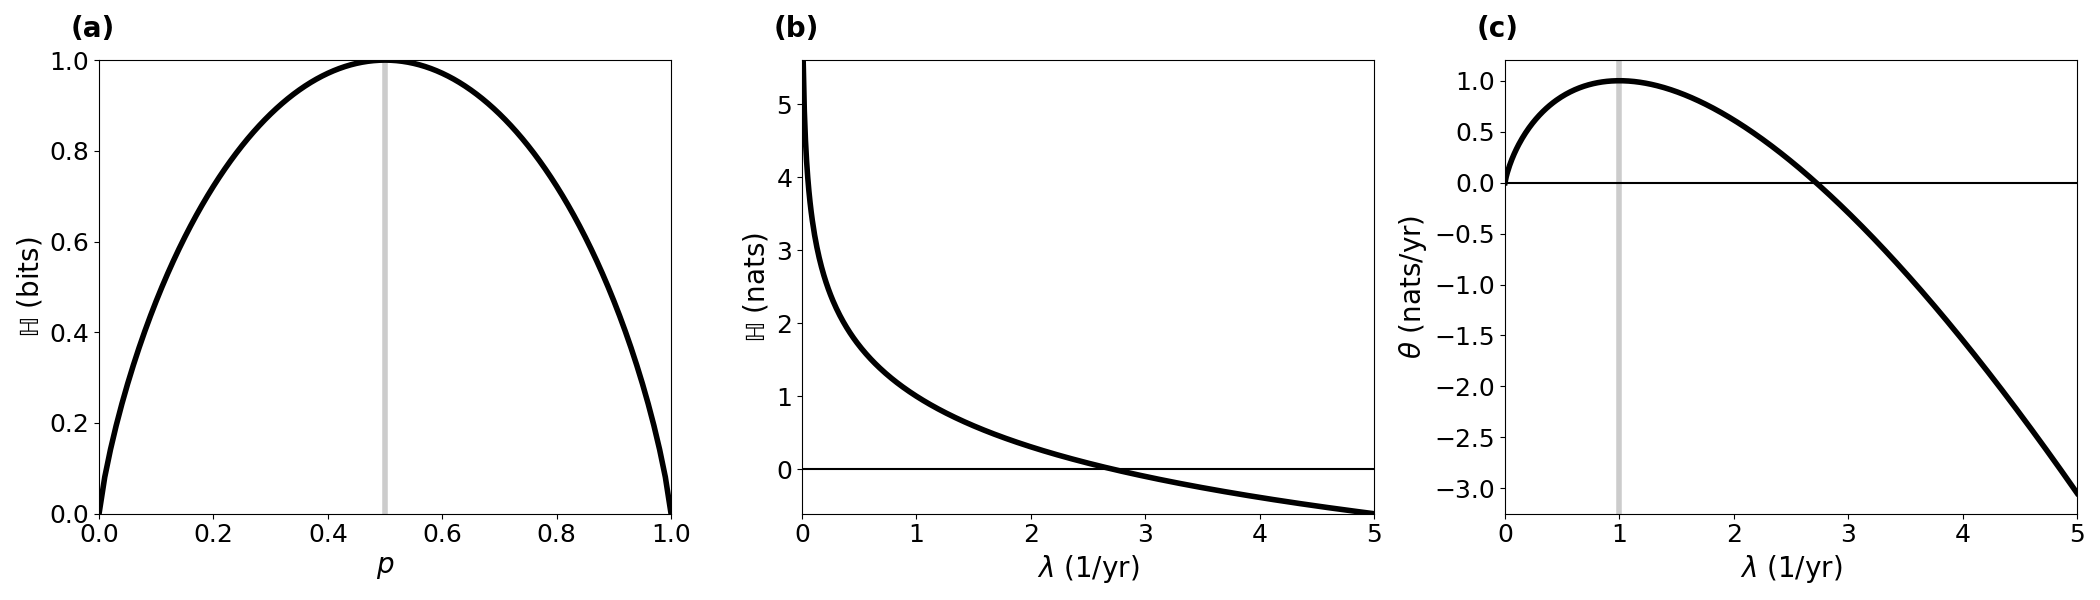
\includegraphics[width=1.0\linewidth]{figs/simple_entropy_py.png}
  \caption{
%   A) Shannon entropy (logarithmic base $2$) of a Bernoulli random variable depending on its success probability $p$.
%   B) Differential entropy with logarithmic base $e$ of an exponentially distributed random variable depending on its rate parameter $\lambda$.
%   C) Entropy rate of a Poisson process with intensity rate $\lambda$.
%   Vertical gray lines indicate the parameter values leading to the highest entropy.
  Shannon entropy of a Bernoulli distribution (a), differential entropy of an exponential distribution (b), and entropy rate of a Poisson process (c).
  Vertical gray lines indicate the parameter values leading to the highest entropy
  }
  \label{fig:simple_entropy}
\end{figure}

We can further consider the \emph{joint entropy} $\H(Y_1,Y_2)$ of two random variables $Y_1$ and $Y_2$, which can be described as 
\begin{equation}
  \H(Y_1,Y_2) = \H(Y_1) + H(Y_2\,|\,Y_1),
\end{equation}
where the \emph{conditional entropy} $H(Y_2\,|\,Y_1)$ describes the uncertainty of $Y_2$ under the condition that $Y_1$ is known.
Note that the joint entropy is symmetric, \ie, $\H(Y_1,Y_2)=\H(Y_2,Y_1)$ and 
\begin{equation}
  \H(Y_1,Y_2)\leq \H(Y_1) + \H(Y_2)
\end{equation}
with equality if $Y_1$ and $Y_2$ are independent.
Consequently, 
\begin{equation}
  \H(Y_2\,|\,Y_1)\leq \H(Y_2)
\end{equation}
with equality in case of independence.

The uncertainty of a stochastic process $Z$ can be measured by its \emph{entropy rate} $\theta(Z)$, which describes the time density of the average information in the process.
For instance, let $Z\sim\Poi(\lambda)$ be a Poisson process with intensity rate $\lambda>0$ describing the moments of occurrence of certain events.
The interarrival times of $Z$ or the times between events are $\Exp(\lambda)$-distributed, such that in the long run on average the time span between events has length $\lambda^{-1}$.
The entropy of the interarrival times is given by $\H(\Exp(\lambda))=1-\log \lambda$, and averaging it over the mean interarrival time gives the entropy rate of the Poisson process $Z$ \citep[Sect.~3.3]{Gaspard1993PR}, \ie,
\begin{equation}
  \theta(Z) = \theta(\Poi(\lambda)) = \lambda\,(1-\log \lambda).
\end{equation}
This entropy rate increases with $\lambda\in[0,\,1]$, reaches its maximum at $1$, and then it decreases (Fig.~\ref{fig:simple_entropy}, panel c).
This behavior is independent of the unit of $\lambda$, because it is based on the differential entropy of the exponential distribution and hence not scale-invariant.
Consequently, it is not an absolute measure of information content, but only useful in comparison to the entropy rates of other stochastic processes.



\subsection{Compartmental systems in equilibrium}\label{sec:one_particle}
Mass-balanced flow of material into a system, within the system and out of the system that consists of several compartments can be modeled by so-called compartmental systems \citep{Anderson1983, Jacquez1993SIAM}.
Compartments are always well-mixed and usually also called \emph{pools} or \emph{boxes}.
One way to describe compartmental systems is by the $d$-dimensional linear ODE system
\begin{equation}\label{eqn:lin_CS_sys}
  \deriv{t}\,\vec{x}(t) = \tens{B}\,\vec{x}(t) + \vec{u},\quad t>0,\\
\end{equation}
with some initial condition $\vec{x}(0) = \vec{x}^0\in\R^d$.
The nonnegative vector $\vec{x}(t)$ describes the amount of material in the different compartments at time $t$, the nonnegative vector $\vec{u}$ is the vector of external inputs to the compartments, and the compartmental matrix $\tens{B}\in\R^{d\times d}$ describes the flux rates between the compartments and out of the system.
The nonnegative off-diagonal value $B_{ij}$ is the flux rate from compartment $j$ to compartment $i$, the absolute value of the negative diagonal value $B_{jj}$ is the total rate of fluxes out of compartment $j$, and the nonnegative value $z_j=-\sum_{i=1}^d B_{ij}$ is the rate of the flux from compartment $j$ out of the system.
By requiring $\tens{B}$ to be invertible we ensure that the system is \emph{open}, \ie, all material that enters the system will eventually also leave it.
Throughout this manuscript, we consider the open compartmental system \eqref{eqn:lin_CS_sys} to have reached its unique steady-state or equilibrium compartment vector $\vec{x}^\ast = -\tens{B}^{-1}\,\vec{u}$.
An open compartmental system in equilibrium given by Eq.\eqref{eqn:lin_CS_sys} is fully characterized by $\vec{u}$ and $\tens{B}$, and we denote it by $M=M(\vec{u},\tens{B})$.


\subsection{The one-particle perspective}
\label{sec:the_one_particle_perspective}
While Eq.~\eqref{eqn:lin_CS_sys} describes the movement of bulk material through the system, compartmental systems in equilibrium can also be described probabilistically by considering the random path of a single particle through the system \citep{Metzler2018MGS}.
If $X_t\in\mathcal{S}:=\{1,2,\ldots,d\}$ denotes the compartment in which the single particle is at time $t$, and $X_t=d+1$ if the particle has already left the system, then $X:=(X_t)_{t\geq0}$ is an absorbing continuous-time Markov chain \citep{Norris1997} on $\widetilde{\mathcal{S}}:=\mathcal{S}\cup\{d+1\}$.
Its initial distribution is given by $\widetilde{\vec{\beta}}=(\beta_1, \beta_2, \ldots, \beta_d, 0)^T$, where $\vec{\beta}:=\vec{u}/\vnorms{\vec{u}}$, and $\beta_j=\P(X_0=j)$ is the probability of the single particle to enter the system through compartment $j$.
The superscript $T$ denotes the transpose of the vector/matrix  and $\vnorms{\vec{u}}=\sum_{i=1}^d |u_i|$ denotes the $l_1$-norm of the vector $\vec{u}$.
The state-transition matrix of $X$ is given by
\begin{equation}\label{eqn:Q}
  \tens{Q} =
  \begin{pmatrix}
    \tens{B} & \vec{0} \\
    \vec{z}^T & 0
  \end{pmatrix},
\end{equation}
and thus
\begin{equation}
  \P(X_t=i) = (e^{t\,\tens{Q}}\,\widetilde{\vec{\beta}})_i = \suml_{j=1}^d (e^{t\,\tens{Q}})_{ij}\,\beta_j, \quad i\in\widetilde{\mathcal{S}},
\end{equation}
is the probability of the particle to be in compartment $i$ at time $t$ if $i\in\mathcal{S}$ or that the particle has left the system if $i=d+1$.
Here, $e^{t\,\tens{Q}}$ denotes the matrix exponential.
Furthermore, 
\begin{equation}
  \P(X_t=i\,|\,X_s=j) = (e^{(t-s)\,\tens{Q}})_{ij},\quad s\leq t,\quad i,j\in\widetilde{\mathcal{S}},
\end{equation}
is the probability that $X$ is in state $i$ at time $t$ given it was in state $j$ at time $s$.
Since the Markov chain $X$ and the compartmental system in equilibrium given by Eq.~\eqref{eqn:lin_CS_sys} are equivalent, we can write
\begin{equation}
  M=M(\vec{u},\tens{B}) = M(X).
\end{equation}


\subsection{The path of a single particle}
A particle's path through the system from the moment of entering until the moment of exit can be described as a sequence of (compartment, sojourn-time)-pairs
\begin{equation}
  \label{eqn:path}
  \mathcal{P}(X) := ((Y_1=X_0, T_1),(Y_2,T_2),\ldots,(Y_{\mathcal{N}-1},T_{\mathcal{N}-1}), Y_{\mathcal{N}}=d+1),
\end{equation}
where $X$ is the absorbing Markov chain associated to the particle's journey.
The sequence $Y_1,Y_2,\ldots,Y_{\mathcal{N}-1}\in\mathcal{S}$ represents the successively visited compartments along with the associated sojourn times $T_1,T_2,\ldots,T_{\mathcal{N}-1}$, the random variable
\begin{equation}
  \mathcal{N}:=\inf\,\{n\in\N:\,Y_n=d+1\}
\end{equation}
denotes the first hitting time of the absorbing state $d+1$ by the \emph{embedded jump chain} $Y:=(Y_n)_{n=1,2,\ldots,\mathcal{N}}$ of $X$ \citep{Norris1997}.
With $\lambda_j:=-Q_{jj}$ the one-step transition probabilities of $Y$ are given by, for $i,j\in\widetilde{\mathcal{S}}$,
\begin{equation}\label{eqn:P_ij}
  P_{ij}:=\P(Y_{n+1}=i\,|\,Y_n=j) = 
  \begin{cases}
    0,\quad & i=j\text{ or }\lambda_j=0,\\
    Q_{ij}/\lambda_j,\quad & \text{else}.
  \end{cases}
\end{equation}
We can also write $\tens{P}=(P_{ij})_{i,j\in\widetilde{\mathcal{S}}}=\tens{Q}\,\tens{D}^{-1} + \tens{I}$, where
\begin{equation}
  \tens{D} := \diag\,(\lambda_1,\lambda_2,\ldots,\lambda_d,\lambda_{d+1})
\end{equation}
is the diagonal matrix with the diagonal entries of $\tens{Q}$ and $\tens{I}$ denotes the identity matrix of appropriate dimension.
We define the matrix $\tens{P}_{\tens{B}} := (P_{ij})_{i,j\in\mathcal{S}}$, then $\tens{M}:=(\tens{I}-\tens{P}_{\tens{B}})^{-1}$ is the \emph{fundamental matrix} of $Y$, with $\tens{I}\in\R^{d\times d}$ denoting the identity matrix.
The entry $M_{ij}$ denotes the expected numbers of visits to compartment $i$ given that the particle entered the system through compartment $j$.
Consequently, the expected number of visits to compartment $i\in\mathcal{S}$ is given by 
\begin{equation}
  \label{eqn:N_i}
  N_i = \suml_{j=1}^d M_{ij}\,\beta_j = (\tens{M}\,\vec{\beta})_i = \left[(\tens{I}-\tens{P}_{\tens{B}})^{-1}\,\vec{\beta}\right]_i 
  = (\tens{D}\,\tens{B}^{-1}\,\vec{\beta})_i
  = \frac{\lambda_i\,x^\ast_i}{\vnorms{\vec{u}}}
\end{equation}
and the total expected number of jumps is given by
\begin{equation}
  \E\left[\mathcal{N}\right] = \suml_{i=1}^d (\tens{M}\,\vec{\beta})_i+1= \suml_{i=1}^d N_i+1,
\end{equation}
where we take into account also the last jump out of the system.

The last jump, $\mathcal{N}$, leads the particle out of the system such that at the moment of this last jump $X$ takes on the value $d+1$.
This last jump happens at the absorption time of the Markov chain $X$, which is defined as
\begin{equation}
   \TT := \inf\,\{t>0: X_t=d+1\}.
\end{equation}
The absorption time is phase-type distributed \citep{Neuts1981}, $\TT\sim\PH(\vec{\beta},\tens{B})$, with \pdf
\begin{equation}
  f_{\TT}(t) = \vec{z}^T\,e^{t\,\tens{B}}\,\vec{\beta},\quad t\geq0.
\end{equation}
It can be shown \citep[Sect.~3.2]{Metzler2018MGS} that the mean or expected value of $\TT$ equals the turnover time \citep{Sierra2016GlobChangBiol} of system \eqref{eqn:lin_CS_sys} in equilibrium and is given by total stocks over total fluxes, \ie, 
\begin{equation}
  \E\left[\TT\right] = \frac{\vnorms{\vec{x}^\ast}}{\vnorms{\vec{u}}}.
\end{equation}
Furthermore, by construction $\sum_{k=1}^{\mathcal{N}-1} T_k = \TT$.
If we denote by $\mathbbm{1}_{\{A\}}$ the indicator function of the logical expression $A$, given by
\begin{equation}
  \mathbbm{1}_{\{A\}} =
  \begin{cases}
    1, \quad A\text{ is true},\\
    0, \quad\text{else},
  \end{cases}
\end{equation}
then $O_j:=\sum_{k=1}^{\mathcal{N}-1} \mathbbm{1}_{\{Y_k=j\}}\,T_k$ is the total time that the particle spends in compartment $j$.
This time is called \emph{occupation time} of $j$ and its mean is given by \citep[Sect.~3.3]{Metzler2018MGS}
\begin{equation}
  \label{eqn:occupation_time}
  \E\left[O_j\right] = \frac{x^\ast_j}{\vnorms{\vec{u}}},
\end{equation}
which induces $\E\left[\TT\right] = \sum_{j=1}^d \E\left[O_j\right]$.


\subsection{Path entropy, entropy rate per unit time, entropy rate per jump}
\label{sec:path_entropy}
The path $\mathcal{P}=\mathcal{P}(X)$ given by Eq.~\eqref{eqn:path} can be interpreted in three different ways.
Each of these ways leads to a different interpretation of the path's entropy.
First, we can look at $\mathcal{P}$ as the result of bookkeeping of the absorbing continuous-time Markov chain $X$, where for all times $t$ we note down the pair $(X_t,t)$ of the current compartment and the current time.
Second, we can consider the path as a discrete-time process.
In each time step $n$, we choose randomly a new compartment $Y_{n+1}$ and an associated sojourn time $T_{n+1}$ of the particle in this compartment.
Third, we can look at $\mathcal{P}$ as a single random variable with values in the space of all possible paths.
Based on the latter interpretation we now derive the path entropy.

We are interested in the uncertainty/information content of the path $\mathcal{P}(X)$ of a single particle.
Along the lines of \citet{Albert1962AMS}, we construct a space $\wp$ that contains all possible paths that can be taken by a particle that runs through the system until it leaves.
Let $\wp_n:=(S\times\R_+)^n\times\{d+1\}$ denote the space of paths that visit $n$ compartments/states before ending up in the environmental compartment/absorbing state $d+1$.
By $\wp:=\bigcup_{n=1}^{\infty}\wp_n$ denote the space of all eventually absorbed paths.
Note that, since $\tens{B}$ is invertible, a path through the system is finite with probability $1$.
Let $l$ denote the Lebesgue measure on $\R_+$ and $c$ the counting measure on $S$.
Furthermore, let $\sigma_n$ be the sigma-finite product measure on $\wp_n$.
It is defined by $\sigma_n:=(c\otimes l)^n \otimes c$.
Almost all sample functions of $(X_t)_{t\geq0}$ can be represented as a point $p\in\wp$ \citep[Chapter~VI]{Doob1953}.
Consequently, we can represent $X$ by a finite-length path $\mathcal{P}(X)=((Y_1,T_1),(Y_2,T_2),\ldots,(Y_n,T_n),Y_{n+1})$ for some $n\in\N$, where $Y_{n+1}=d+1$.

For each set $W\subseteq\wp$ for which $W\cap \wp_n$ is $\sigma_n$-measurable for each $n\in\N$, we define $\sigma^\ast(W) := \sum_{n=1}^{\infty} \sigma_n(W\cap\wp_n)$.
This measure is defined on the $\sigma$-field $\mathcal{F}^\ast$ which is the smallest $\sigma$-field containing all sets $W\subseteq\wp$ whose projection on $\R^n_+$ is a Borel set for each $n\in\N$.
Let $\sigma$ be a measure on all sample functions, defined for all subsets $W$ whose intersection with $\wp$ is in $\mathcal{F}^\ast$. 
We define it by $\sigma(W):=\sigma^*(W\cap\wp)$.

Let $p=((x_1,t_1),(x_2,t_2,),\ldots,(x_n,t_n),d+1)\in\wp$ for some $n\in\N$.
For $i\neq j$, denote by $N_{ij}(p)$ the total number of path $p$'s one-step transitions from $j$ to $i$ and by $R_j(p)$ the total amount of time spent in $j$.

\begin{mytheorem}\label{theorem:path_pdf}
	The \pdf\ of $\mathcal{P}=\mathcal{P}(X)$ with respect to $\sigma$ is given by
	\begin{equation}
    \begin{aligned}
      f_{\mathcal{P}}(p) = \beta_{x_1}\Bigg(\prodl_{j=1}^d\,\prodl_{i=1,i\neq j}^{d+1} &(Q_{ij})^{N_{ij}(p)}\Bigg)\prodl_{j=1}^d e^{-\lambda_j\,R_j(p)},\\
      & p=((x_1,t_1),(x_2,t_2),\ldots,(x_n,t_n),d+1)\in\wp.
    \end{aligned}
	\end{equation}
\end{mytheorem}

\begin{proof}
	Let $x_1,x_2,\ldots,x_n\in S$, $x_{n+1}=d+1$, and $t_1,t_2,\ldots,t_n\in\R_+$.
	Since
	\begin{equation}
    \begin{aligned}
      &\P((Y_1=x_1,T_1\leq t_1),\ldots,\,(Y_n=x_n,T_n\leq t_n),\, Y_{n+1}=d+1) \\
% 		&\qquad= \P(Y_{n+1}=d+1\,|\,Y_n=x_n)\,\prodl_{k=1}^n \P(Y_k=x_k,T_k\leq t_k\,|\,Y_{k-1}=x_{k-1})\\
      &\qquad= \P(Y_{n+1}=d+1\,|\,Y_n=x_n)\\
      &\qquad\qquad\cdot\,\prodl_{k=2}^n \P(Y_k=x_k,T_k\leq t_k\,|\,Y_{k-1}=x_{k-1})\,\P(Y_1=x_k,T_1\leq t_1)\\
      &\qquad= P_{d+1,x_n}\left[\prodl_{k=2}^n P_{x_{k} x_{k-1}}\left(1-e^{-\lambda_{x_k}\,t_k}\right)\right] \beta_{x_1}\left(1-e^{-\lambda_{x_1}\,t_1}\right)\\
      &\qquad= \intl_{\mathbb{T}_n} \beta_{x_1}\prodl_{k=1}^n Q_{x_{k+1}x_k}\,e^{-\lambda_{x_k}\,\tau_k}\,\mathrm{d}\tau_1\mathrm{d}\tau_2\cdots\mathrm{d}\tau_n
    \end{aligned}
  \end{equation}
	with $\mathbb{T}_n=\{(\tau_1,\tau_2,\ldots,\tau_n)\in\R^n_+:\,0\leq\tau_1\leq t_1,0\leq\tau_2\leq t_2,\ldots,0\leq\tau_n\leq t_n\}$,
	the \pdf\ of $\mathcal{P}=\mathcal{P}(x)$ with respect to $\sigma$ is given by
	\begin{equation}
    \begin{aligned}
      f_{\mathcal{P}}(p) = \beta_{x_1}\prodl_{k=1}^n &Q_{x_{k+1}x_k}\,e^{-\lambda_{x_k}\,t_k},\\
      & p=((x_1,t_1),(x_2,t_2),\ldots,(x_n,t_n),d+1)\in\wp.
    \end{aligned}
  \end{equation}
	The term $Q_{x_{k+1}x_k}=Q_{ij}$ enters exactly $N_{ij}(p)$ times.
	Furthermore,
	\begin{equation}
    \begin{aligned}
      \prodl_{k=1}^n e^{-\lambda_{x_k}\,t_k} &= \prodl_{k=1}^n\,\prodl_{j=1}^d \mathbbm{1}_{\{x_k=j\}}\,e^{-\lambda_j\,t_k}
      = \prodl_{j=1}^d e^{-\lambda_j\,\suml_{k=1}^n \mathbbm{1}_{\{x_k=j\}}\,t_k}\\
      &= \prodl_{j=1}^d e^{-\lambda_j\,R_j(p)}.
    \end{aligned}
  \end{equation}
	We make the according substitutions and the proof is finished.
\end{proof}

The entropy of the absorbing continuous-time Markov chain $X$ is equal to its entropy on the random but finite time horizon $[0,\,\TT]$, which in turn equals the entropy of a single particle's path $\mathcal{P}$ through the system.

\begin{mytheorem}\label{thm:entropy_of_X}
	The entropy of the absorbing continuous-time Markov chain $X$ is given by
	\begin{equation}
    \label{eqn:H_X}
    \begin{aligned}
      \H(X) &= \H(\mathcal{P})\\
      &= -\suml_{i=1}^d\beta_i\,\log\beta_i\\
      &\quad + \suml_{j=1}^d \frac{x^\ast_j}{\vnorms{\vec{u}}}\left[\suml_{i=1,i\neq j}^d \,B_{ij}\,(1-\log B_{ij}) + z_j\,(1-\log z_j)\right].
    \end{aligned}
	\end{equation}
\end{mytheorem}

\begin{proof}
	Let $X$ have the finite path representation 
	\begin{equation}
		\mathcal{P}=\mathcal{P}(X)=((Y_1,T_1),(Y_2,T_2),\ldots,(Y_n,T_n),d+1)
	\end{equation}
	for some $n\in\N$, and denote by $f_{\mathcal{P}}$ its \pdf.
	Then, by Theorem~\ref{theorem:path_pdf},
	\begin{equation}
		-\log f_{\mathcal{P}}(\mathcal{P}) = -\log\beta_{Y_1} - \suml_{j=1}^d\,\suml_{i=1,i\neq j}^{d+1}N_{ij}(\mathcal{P})\,\log Q_{ij} + \suml_{j=1}^d \lambda_j\,R_j(\mathcal{P}).
	\end{equation}
	We compute the expectation and get
	\begin{equation}
    \begin{aligned}
      \H(X) &= \H(\mathcal{P}) = -\E\left[\log f_{\mathcal{P}}(\mathcal{P})\right]\\
      &= -\E\left[\log\beta_{Y_1}\right] - \suml_{j=1}^d\,\suml_{i=1,i\neq j}^{d+1}\E\left[N_{ij}(\mathcal{P})\right]\,\log Q_{ij} + \suml_{j=1}^d \lambda_j\,\E\left[R_j(\mathcal{P})\right]\\
      &= \H(Y_1) + \suml_{j=1}^d \lambda_j\,\E\left[R_j(\mathcal{P})\right] - \suml_{j=1}^d\,\suml_{i=1,i\neq j}^{d+1}\E\left[N_{ij}(\mathcal{P})\right]\,\log Q_{ij}.
    \end{aligned}
  \end{equation}
	Obviously, $\E\left[R_j(\mathcal{P})\right]=\E\left[O_j\right]=x^\ast_j/\vnorms{\vec{u}}$ is the mean occupation time of compartment $j\in S$ by $X$.
	Furthermore, for $i\in\widetilde{S}$ and $j\in S$ such that $i\neq j$, by Eqs.~\eqref{eqn:N_i} and~\eqref{eqn:P_ij},
	\begin{equation}
		\E\left[N_{ij}(\mathcal{P})\right] = \E\left[N_j(\mathcal{P})\right]\,P_{ij} = 
		\begin{cases}
			\frac{x^\ast_j}{\vnorms{\vec{u}}}\,B_{ij},\quad & i\leq d,\\
			\frac{x^\ast_j}{\vnorms{\vec{u}}}\,z_j,&i=d+1.
		\end{cases}
	\end{equation}
	Together with $\lambda_j=\sum_{i=1,i\neq j}^{d} B_{ij}+z_j$, we obtain
	\begin{equation}
    \begin{aligned}
      \H(X) &= \H(Y_1)+ \suml_{j=1}^d \frac{x^\ast_j}{\vnorms{\vec{u}}}\Bigg[\left(\suml_{i=1,i\neq j}^d B_{ij}+z_j\right)\\
      &\qquad\qquad\qquad\qquad - \suml_{i=1,i\neq j}^d B_{ij}\,\log B_{ij} - z_j\,\log z_j\Bigg]\\
      &= -\suml_{i=1}^d \beta_i\log\beta_i + \suml_{j=1}^d \frac{x^\ast_j}{\vnorms{\vec{u}}} \Bigg[\suml_{i=1,i\neq j}^d B_{ij}\,(1-\log B_{ij})\\
      &\qquad\qquad\qquad\qquad\qquad + z_j\,(1-\log z_j)\Bigg].
    \end{aligned}
  \end{equation}
\end{proof}

By some simple substitutions and rearrangements, we obtain two representations of $\H(X)=\H(\mathcal{P})$ that are easy to interpret.
For simplicity of notation, we define
\begin{equation}
  \H(\vec{\beta}) := -\suml_{i=1}^d\beta_i\,\log\beta_i.
\end{equation}

\begin{myproposition}\label{prop:entropy_of_X}
	The entropy of the absorbing continuous-time Markov chain $X$ is also given by
	\begin{equation}
	  \label{eqn:H_occupation_time}
	  \H(X) = \H(\vec{\beta}) + \suml_{j=1}^d \E\left[O_j\right] \left(\suml_{i=1,\,i\neq j}^d \theta(\Poi(B_{ij})) + \theta(\Poi(z_j))\right)
	\end{equation}
	and
	\begin{equation}
	  \label{eqn:H_number_of_visits}
	  \begin{aligned}
      \H(X)& = \H(\vec{\beta})\\
      &\quad + \suml_{j=1}^d \E\left[N_j\right]\, \left(\H(\Exp(\lambda_j)) + \H(P_{1,j}, P_{2, j},\ldots,P_{d, j}, P_{d+1,j})\right),
    \end{aligned}
  \end{equation}
  which can be rewritten as
  \begin{align}
    \H(X) & = \H(\vec{\beta}) + \suml_{j=1}^d \E\left[N_j\right]\, \H(P_{1,j}, P_{2, j},\ldots,P_{d, j}, P_{d+1,j}) \label{eqn:H_discrete} \\
    &\quad + \suml_{j=1}^d \E\left[N_j\right]\, \H(\Exp(\lambda_j)).\label{eqn:H_continuous}      
  \end{align}
\end{myproposition}

\begin{proof}
  By virtue of Eq.~\eqref{eqn:H_occupation_time} we replace $x^\ast_j/\vnorms{\vec{u}}$ by $\E\left[O_j\right]$ in Eq.~\eqref{eqn:H_X} and take into account that the entropy rate of a Poisson process with intensity rate $\lambda$ equals $\lambda\,(1-\log \lambda)$ to prove Eq.~\eqref{eqn:H_occupation_time}.
  To prove Eq.~\eqref{eqn:H_number_of_visits} we use Eq.~\eqref{eqn:N_i} to replace $x^\ast_j/\vnorms{\vec{u}}$ in Eq.~\eqref{eqn:H_X} by $\E\left[N_j\right]/\lambda_j$ and obtain
  \begin{equation}
    \begin{aligned}
      \H(X) &= -\suml_{i=1}^d\beta_i\,\log\beta_i + \suml_{j=1}^d \E\left[N_j\right](1-\log \lambda_j)\\
      &\qquad +\suml_{j=1}^d \E\left[N_j\right]\left(- \suml_{i=1,i\neq j}^d \frac{B_{ij}}{\lambda_j}\,\log \frac{B_{ij}}{\lambda_j} - \frac{z_j}{\lambda_j}\,\log \frac{z_j}{\lambda_j}\right).
    \end{aligned}
	\end{equation}
	Here, $(1-\log \lambda_j)$ is the entropy of an exponential random variable with rate parameter $\lambda_j$.
	Using definition \eqref{eqn:P_ij} of $P_{ij}$ we replace $B_{ij}/\lambda_j$ by $P_{ij}$ for $i\in\mathcal{S}$ and $z_j/\lambda_j$ by $P_{d+1,j}$ and finish the proof.
\end{proof}

We now define the \emph{path entropy} of the compartmental system $M$ in equilibrium, given by Eq.~\eqref{eqn:lin_CS_sys}, as the path entropy of its associated continuous-time Markov chain $X$, \ie
\begin{equation}
  \H(M):=\H(X)=\H(\mathcal{P}(X)).
\end{equation}
For a one-dimensional compartmental system $M_\lambda$ in equilibrium with rate $\lambda>0$ and positive external input given by
\begin{equation}
  \deriv{t}\,x(t) = -\lambda\,x(t) + u,\quad t>0,
\end{equation}
the entropy of the initial distribution vanishes, and we obtain
\begin{equation}
  \H(M_\lambda) = \frac{x^\ast}{u}\,\lambda\,(1-\log\,\lambda) = \frac{1}{\lambda}\,\lambda\,(1-\log\,\lambda) = 1-\log\,\lambda,
\end{equation}  
which equals the differential entropy $1-\log\lambda$ of the exponentially distributed mean transit time $\TT_\lambda\sim\Exp(\lambda)$, reflecting that the only uncertainty of the particle's path in a one-pool system is the time of the particle's exit.
The exponential distribution with rate parameter $\lambda$ is the distribution of the interarrival time of a Poisson process wit intensity rate $\lambda$.
Hence, we can interpret $\H(M_\lambda) = \lambda^{-1}\,\lambda\,(1-\log\lambda)$ as the instantaneous Poisson entropy rate $\lambda\,(1-\log\lambda)$ multiplied with the expected duration $\E\left[\TT\right]=\lambda^{-1}$ of the particle's stay in the system.

Migrating to a $d$-dimensional system, we can interpret $\H(M)$ as the entropy of a continuous-time process in the light of Eq.~\eqref{eqn:H_occupation_time} and as the entropy of a discrete-time process in the light of Eq.~\eqref{eqn:H_number_of_visits}.
In both interpretations, the first term $\H(\vec{\beta})=\H(X_0)=\H(Y_1)$ represents the uncertainty of the first pool through which the particle enters the system.
In the continuous-time interpretation, the uncertainty of the subsequent travel is the weighted average of the superposition of $d$ Poisson processes describing the instantaneous uncertainty of possible jumps of the particle inside the system, $\theta(\Poi(B_{ij}))$, and out of the system, $\theta(\Poi(z_j))$, where the weights are the expected occupation times of the different compartments $j\in\mathcal{S}$. 
In the discrete-time interpretation, the subsequent travel's uncertainty is the average of uncertainties associated to each pool, weighted by the number of visits to the respective pools.
The uncertainty associated to each pool comprises the uncertainty of the length of the stay in the pool, $\H(\Exp(\lambda_j))$, and the uncertainty of where to jump afterwards, $\H(\{P_{ij}:\,i\in\widetilde{\mathcal{S}},\,j\in\mathcal{S},i\neq j\})$.
Hence, in the light of Eq.~\eqref{eqn:H_number_of_visits}, we can separate the path entropy into a discrete part associated to jump uncertainty given by Eq.~\eqref{eqn:H_discrete} and a continuous part associated to sojourn time uncertainty given by Eq.~\eqref{eqn:H_continuous}.

The two interpretations of the path entropy $\H(M)$ (as a continuous-time or discrete-time process) motivate two different entropy rates as described earlier.
The \emph{entropy rate per unit time} is given by
\begin{equation}
  \theta(M) = \frac{\H(M)}{\E\left[\TT\right]}
\end{equation}
and the \emph{entropy rate per jump} by
\begin{equation}
  \theta_J(M) = \frac{\H(M)}{\E\left[\mathcal{N}\right]}.
\end{equation}
While the path entropy measures the uncertainty of the entire path, entropy rates measure the average uncertainty of the instantaneous future of a particle while it is in the system: for the entropy rate per unit time the uncertainty entailed by the infinitesimal future, and for the entropy rate per jump the uncertainty entailed by the next jump.


\subsection{The maximum entropy principle (MaxEnt)}
MaxEnt arose in statistical mechanics as a variational principle to predict the equilibrium states of thermal systems and later was applied to matters of information and as a general procedure to draw inferences based on self-consistency requirements \citep{Presse2013RMP}.
Its relationship to information theory and stochastics was established by \citet{Jaynes1957PR1, Jaynes1957PR2}.
The general idea is to identify the most uninformed probability distribution to represent some given data in the sense that the maximum entropy distribution, constrained to given data, uses the information provided by the data only and nothing else.
This approach ensures that no additional subjective information creeps into the distribution.
The goal of this section is to transfer MaxEnt to compartmental systems in order to identify the compartmental system that represents our state of knowledge best in different situations, and at the same time get a better understanding of the introduced entropy measures.

\begin{example}
\label{max_ent_example_1}
Consider the set $\mathcal{M}_1$ of equilibrium compartmental systems~\eqref{eqn:lin_CS_sys} with a predefined nonzero input vector $\vec{u}$, a predefined mean transit time $\E\left[\TT\right]$, and an unknown steady-state vector $\vec{x}^\ast$ comprising nonzero components.
We are interested in the most unbiased compartmental system that reflects our state of information, where maximum unbiasedness is achieved by identifying $M^\ast_1\in\mathcal{M}_1$ such that the entropy rate per unit time $\theta(M^\ast_1)$, or equivalently the path entropy $\H(\mathcal{P}(M^\ast_1))$, is maximized. 
We can show (see Proposition~\ref{proposition:max_ent_example_1}) that the compartmental system $M^\ast_1=M(\vec{u},\tens{B})$ with 
\begin{equation}
	\tens{B} = \begin{pmatrix}
    -\lambda & 1 & \cdots & 1\\
		1 & -\lambda & 1 \cdots & 1 \\
		\vdots & & \ddots & \vdots\\
		1 & \cdots & 1 & -\lambda
  \end{pmatrix},
\end{equation}
where $\lambda=d-1+1/\E\left[\TT\right]$, 		
is the maximum entropy model in $\mathcal{M}_1$.
In the special case $d=1$ for a one-dimensional compartmental system, we obtain $B=-1/\E\left[\TT\right]$.
Since in this case $\TT\sim\Exp(-B)$, we see that the exponential distribution is the maximum entropy distribution in the class of all nonnegative continuous probability distributions with fixed expected value.
This special case is very well known \citep[Example~12.2.5]{Cover2006}.
\end{example}

\begin{example}
\label{max_ent_example_2}
Let us consider the sub§class $\mathcal{M}_2\subseteq\mathcal{M}_1$ of compartmental models from the previous example with the additional restriction of a predefined positive steady-state vector $\vec{x}^\ast$.
Then the compartmental system $M^\ast_2=M(\vec{u},\tens{B})$ with
\begin{equation}
	B_{ij} = \begin{cases}
    \sqrt\frac{x_i^\ast}{x_j^\ast},\quad & i\neq j,\\
		-\suml_{k=1,k\neq j}^d \sqrt\frac{x_k^\ast}{x_j^\ast} - \frac{1}{\sqrt{x_j^\ast}}, \quad &i=j,
		\end{cases}
  \end{equation}
is the maximum entropy model in $\mathcal{M}_2$ (see Proposition~\ref{proposition:max_ent_example_2}).
\end{example}

\subsection{Structural model identification via MaxEnt}
Suppose we observe a natural system and conduct measurements from which we try to construct a linear autonomous compartmental model in equilibrium that represents the observed natural system as well as possible.
The first question that arises is the one for the number of compartments the model should ideally have.
MaxEnt cannot be helpful here because by adding more and more compartments we can theoretically increase the entropy of the model indefinitely.
Consequently, the problem of finding the right dimension of system~\eqref{eqn:lin_CS_sys} has to be solved by other means.
One way to do this is to analyze an impulse response function of the system and its Laplace transform, \ie\ the transfer function of the system, and identify the most dominating frequencies.
The impulse response or the transfer function might be possible to obtain by tracer experiments \citep{Anderson1983, Walter1986MBS}.

In \citet[Chapter~16]{Anderson1983} the \emph{structural identification problem} of linear autonomous systems is described as follows.
Suppose we are interested in determining a $d$-dimensional system of form~\eqref{eqn:lin_CS_sys}.
We are interested in sending an impulse into the system at time $t=0$ and analyzing its further behavior.
To that end, we rewrite the system to
\begin{equation}\label{eqn:ABC_system}
	\begin{aligned}
		\deriv{t}\,\vec{x}(t) &= \tens{B}\,\vec{x}(t) + \tens{A}\,\vec{u},	\quad t\geq0,\\
		\vec{x}(0) &= \vec{0}\in\R^d,\\
		\vec{y}(t) &= \tens{C}\,\vec{x}(t),\quad t\geq0.
	\end{aligned}
\end{equation}
Note that the roles of $\tens{A}$ and $\tens{B}$ are interchanged here with respect to \citet{Anderson1983}.
In a typical tracer experiment, we choose an input vector $\vec{u}$ and the \emph{input distribution matrix} $\tens{A}$, which defines how the input vector enters the system.
Then we decide which compartments we can observe to determine the \emph{output connection matrix} $\tens{C}$.
The experiment is now to inject an impulse into the system and to record the output function $\vec{y}(t) =\tens{C}\,\vec{x}(t)$.
\citet{Bellman1970MBS} pointed out that the input-output relation is given by
\begin{align*}
	\vec{y}(t) &= \tens{C}\,\vec{x}(t) = \tens{C}\,\intl_0^t e^{(t-\tau)\,\tens{B}}\,\tens{A}\,\vec{u}(\tau)\dd{\tau}\\
	&= \left[\tens{C}\,e^{t\,\tens{B}}\,\tens{A}\right] * \vec{u}(t),
\end{align*}
where $*$ is the convolution operator.
The model parameters enter the input-output relation only in the matrix-valued \emph{impulse response function}
\begin{equation}
	\tens{\Psi}(t):=\tens{C}\,e^{t\,\tens{B}}\,\tens{A},\quad t\geq0,
\end{equation}
or in the \emph{transfer function}
\begin{equation}
	\widehat{\tens{\Psi}}(s) := \tens{C}\,(s\,\tens{I}-\tens{B})^{-1}\,\tens{A}, \quad s\geq0,
\end{equation}
which is the Laplace transform matrix of $\tens{\Psi}$.
Consequently, all identifiable parameters of $\tens{A}$, $\tens{B}$, and $\tens{C}$ must be identified through $\tens{\Psi}$ or $\widehat{\tens{\Psi}}$.
Difficulties arise because the entries of the matrices $\tens{\Psi}$ and $\widehat{\tens{\Psi}}$ are usually nonlinear expressions of the elements of $\tens{A}$, $\tens{B}$, and $\tens{C}$.
We call system~\eqref{eqn:ABC_system} \emph{identifiable} if this nonlinear system of equations has a unique solution $(\tens{A},\tens{B},\tens{C})$ for given $\tens{\Psi}$ or $\widehat{\tens{\Psi}}$.
Otherwise the system is called \emph{nonidentifiable}.
Usually, the matrices $\tens{A}$ and $\tens{C}$ are already know from the experiment's setup.
What remains is to identify the compartmental matrix $\tens{B}$, and this can be done by MaxEnt.

 
\section{Application to particular systems}
First, we apply the presented theory to some equilibrium compartmental models with very simple structure in order to get some grasp on the new entropy concept.
Then we compute entropy quantities for two carbon-cycle models in dependence on environmental and biochemical parameters.
Afterwards, we apply MaxEnt to solve an equifinality problem in model selection.

\subsection{Simple examples}
\label{sec:simple_examples}
From Table~\ref{fig:entropy_table} we can see that depending on the connections between compartments smaller systems can have greater path entropy and entropy rates than bigger systems, even though systems with more compartments can theoretically reach higher entropy.
Furthermore, we see from the depicted examples that the system with the highest path entropy does neither have the highest entropy rate per unit time nor per jump.
Adding connections to a system, one would expect higher path entropy, but the path entropy might actually decrease because the new connections potentially provide a faster way out the system.

\begin{table}[htbp]
  \centering
  \includegraphics[width=1.0\linewidth]{figs/entropy_table.png}
  \caption{Overview of different entropy measures of simple models with different structures.
%   The columns from left to right represent a schematic of the model, its mathematical representation, its entropy rate per jump, its mean number of jumps, its entropy rate per unit time, its mean transit time, and its path entropy.
  Underlined numbers are the highest values per column
  }
  \label{fig:entropy_table}
\end{table}


\subsection{A linear autonomous global carbon-cycle model}
\label{sec:example_1}
We consider the global carbon-cycle model introduced by \citet{Emanuel1981} (Fig.~\ref{fig:Emanuel_model}).
% \begin{SCfigure}%[htbp]
\begin{figure}[htbp]
  \centering
  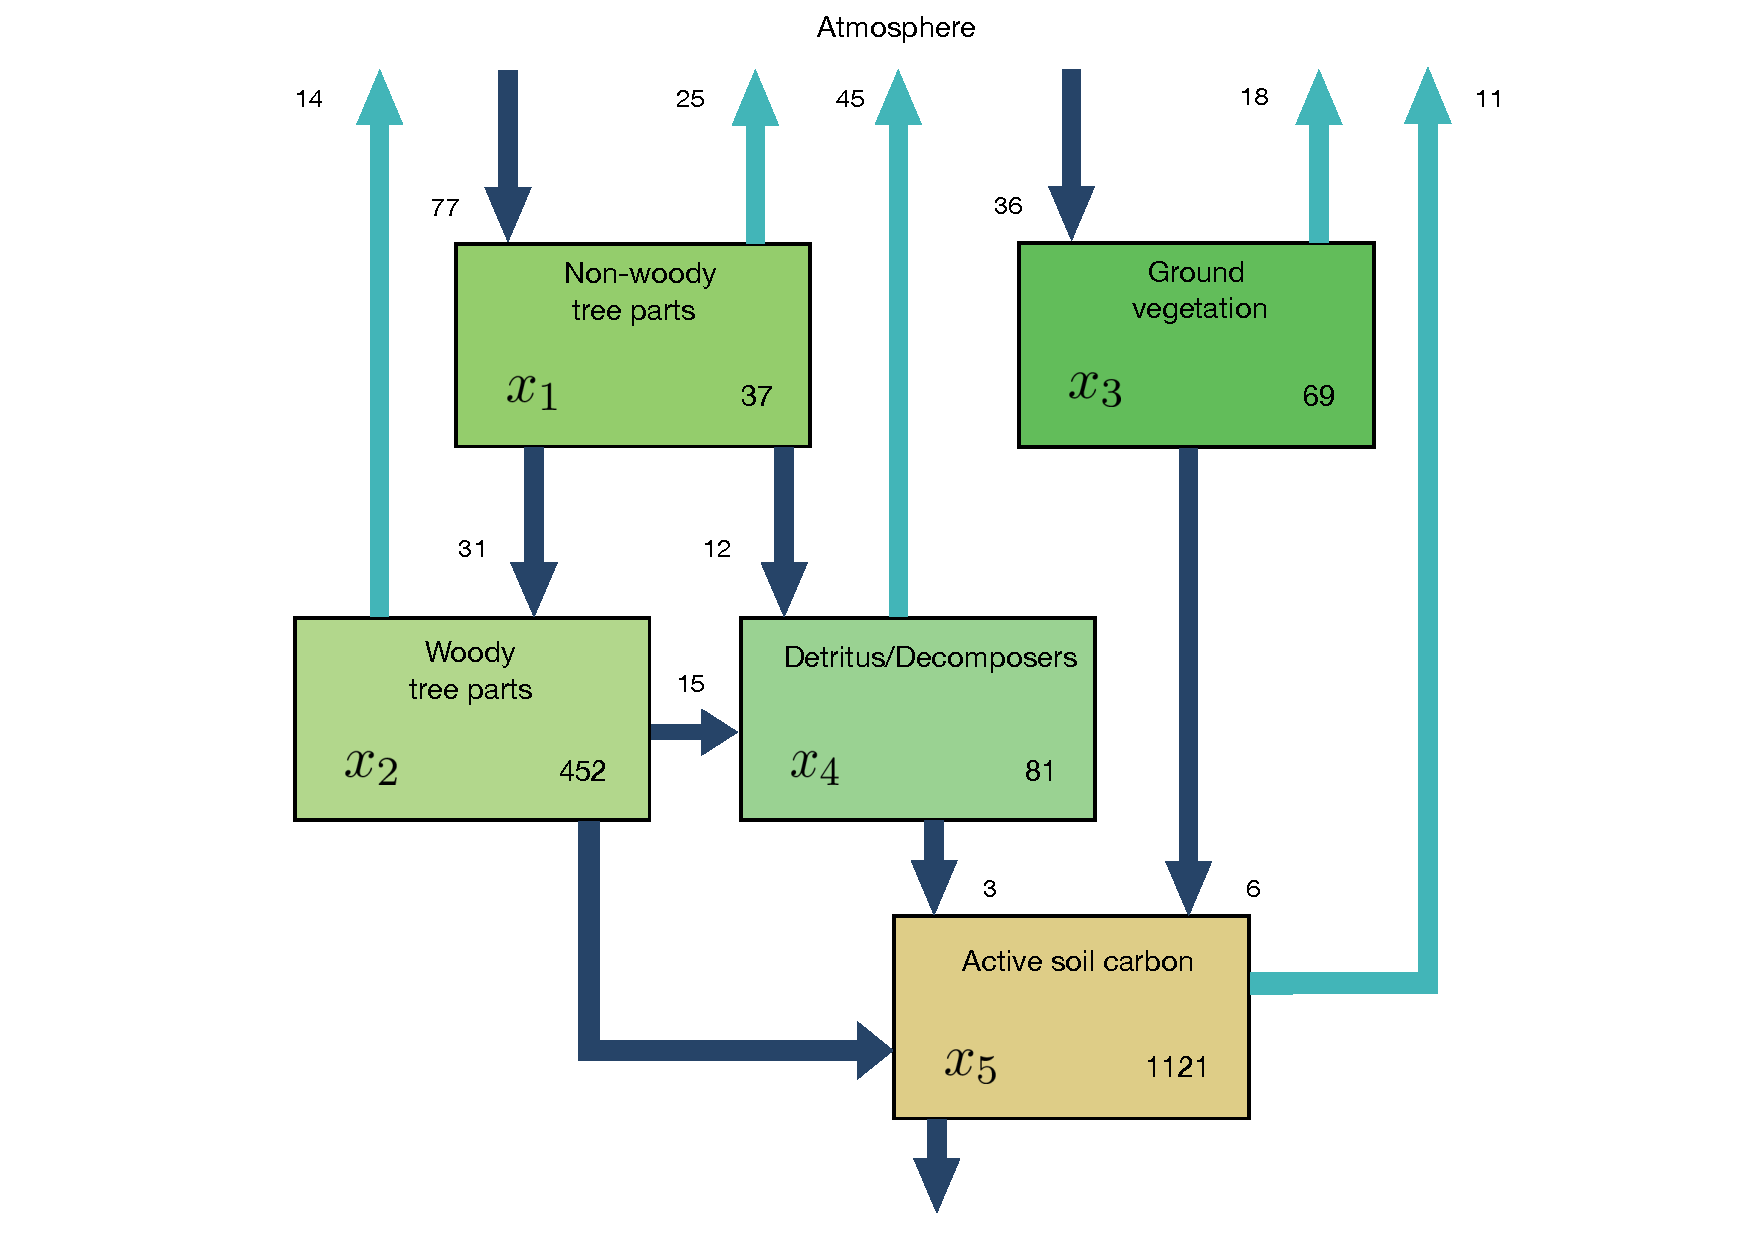
\includegraphics[width=0.5\linewidth]{figs/EmanuelModelStructure.pdf}
  \caption{Schematic of the linear autonomous global carbon cycle model in steady state introduced by \citet{Emanuel1981}
%     The model comprises five compartments: non-woody tree parts $x_1$ ($37\,\peta\gC$), woody tree parts $x_2$ ($452\,\peta\gC$), ground vegetation $x_3$ ($69\,\peta\gC$), detritus/decomposers $x_4$ ($81\,\peta\gC$), and active soil carbon $x_5$ ($1,121\,\peta\gC$). The atmosphere (1) is considered to be outside of the modeled system but provides the system with external inputs and receives external outputs from it. Numbers next to arrows indicate fluxes between compartments in $\peta\gC\,\yr^{-1}$.
  }
  \label{fig:Emanuel_model}
% \end{SCfigure}
\end{figure}
The model comprises five compartments: non-woody tree parts $x_1=37\,\peta\gC$, woody tree parts $x_2=452\,\peta\gC$, ground vegetation $x_3=69\,\peta\gC$, detritus/decomposers $x_4=81\,\peta\gC$, and active soil carbon $x_5=1,121\,\peta\gC$.
We introduce an environmental rate modifier $\xi$ which controls the speed of the system.
This parameter could potentially increase and speed up the system with increasing global surface temperature.
For a given $\xi$ the equilibrium model $M_\xi=M(\vec{u},\,\tens{B}_\xi)$ is given by
\begin{equation}
  \vec{u} = (77;\,0;\,36;\,0;\,0)^{\transpose}\, \peta\gC\,\yr^{-1}
\end{equation}
and
\begin{equation}
    \tens{B}_\xi = \xi\,\left(\begin{matrix}
      -77/37 &       0 &      0 &      0 & 	  0\\
       31/37 & -31/452 &      0 &      0 & 	  0\\
	   0 &       0 & -36/69 &      0 & 	  0\\
       21/37 &  15/452 &  12/69 & -48/81 & 	  0\\
	   0 &   2/452 &   6/69 &   3/81 & -11/1,121
	 \end{matrix}\right)\,\yr^{-1},
\end{equation}
where the numbers are chosen as in \citet{Thompson1999GCB}. 
The input vector is expressed in units of petagrams of carbon per year ($\peta\gC\,\yr^{-1}$) and the fractional transfer coefficients in units of per year ($\yr^{-1}$).
Because $\tens{B}_\xi$ is a lower triangular matrix, the model contains no feedbacks.
For every value of $\xi$ the system has a different steady state (Fig.~\ref{fig:Emanuel_entropies}, panel (a)).
The higher the value of $\xi$, the faster the system, which makes the mean transit time (panel (b)) decrease, and because of shorter paths also the path entropy (panel (d)) decreases.
Since $\xi$ has no impact on the structure of the model, the mean number of jumps (panel (c)) remains unaffected.
This can also be seen from the solid line marked by squares in panel (d)).
It represents the part of the path entropy related to jump-associated uncertainties (Eq.~\eqref{eqn:H_discrete}).
The solid line marked by circles represents the part of the path entropy related to sojourn-associated uncertainties (Eq.~\eqref{eqn:H_continuous}), which as a weighted average of one-pool entropies decreases similar to the entropy of an exponential distribution with increasing rate parameter $\lambda$ (Fig.~\ref{fig:simple_entropy}, panel (b)).
The two parts together constitute the path entropy as represented by the unmarked solid line.

The entropy rate per unit time (panel (e)) increases until $\xi\approx6$ and decreases afterwards, because with increasing system speed the uncertainty associated to sojourn times more and more dominates the uncertainty associated to jumps.
While the uncertainty associated to jumps averaged over the path length increases because the total jump uncertainty is constant (see solid line marked with squares in panel (d) and the mean path length decreases (panel (b)), the sojourn-associated uncertainty decreases with increasing system speed for $\xi>6$ similar to the entropy rate of a Poisson process with intensity rate $\lambda>1$.
The entropy rate per jump (panel f) decreases with increasing $\xi$, because the path entropy of the system decreases.

Dashed lines in panels (d)--(f) show the respective entropy values for a one-pool system $M_\lambda=M((77+36)\,\peta\gC\,\yr^{-1},\, -\lambda)$ with the same mean transit time, \ie\ $\lambda^{-1} = \E\left[\TT_\xi\right]$.
The solid and dashed lines intersect at $\xi\approx4.31$ in panels (d) and (e).
Before this break-even point the path of the Emanuel model is harder to predict than the path (\ie\ the exit time of the particle) of a one-pool model with the same mean transit time.
After this point of break even, the path of the Emanuel model with five compartments is easier to predict than only the transit time in a one-pool model.
The reason is that as the system becomes faster, the differential entropy of the sojourn times in slow pools decreases so fast that at some point the sojourn times in slow pools visited by few particles becomes rather unimportant.
The one-pool model's path becomes relatively harder to predict because it puts too much weight on a small amount of slowly cycling particles.

Note that there is no point in comparing jump-associated uncertainties (square-marked lines) with one-pool entropies (dashed lines), because the former are discrete entropies and the latter differential entropies.
Comparison of a differential entropy with another quantity becomes only reasonable if a second differential entropy is involved as is true for the path entropy or the entropy rates $\theta$ and $\theta_J$ (unmarked solid lines).
Hence, square- and circle-marked lines assist in understanding the composition of the entropies of the multi-pool system, and only the composition of the two can then be compared to the one-pool entropy rate.


\begin{figure}[htbp]
    \centering
    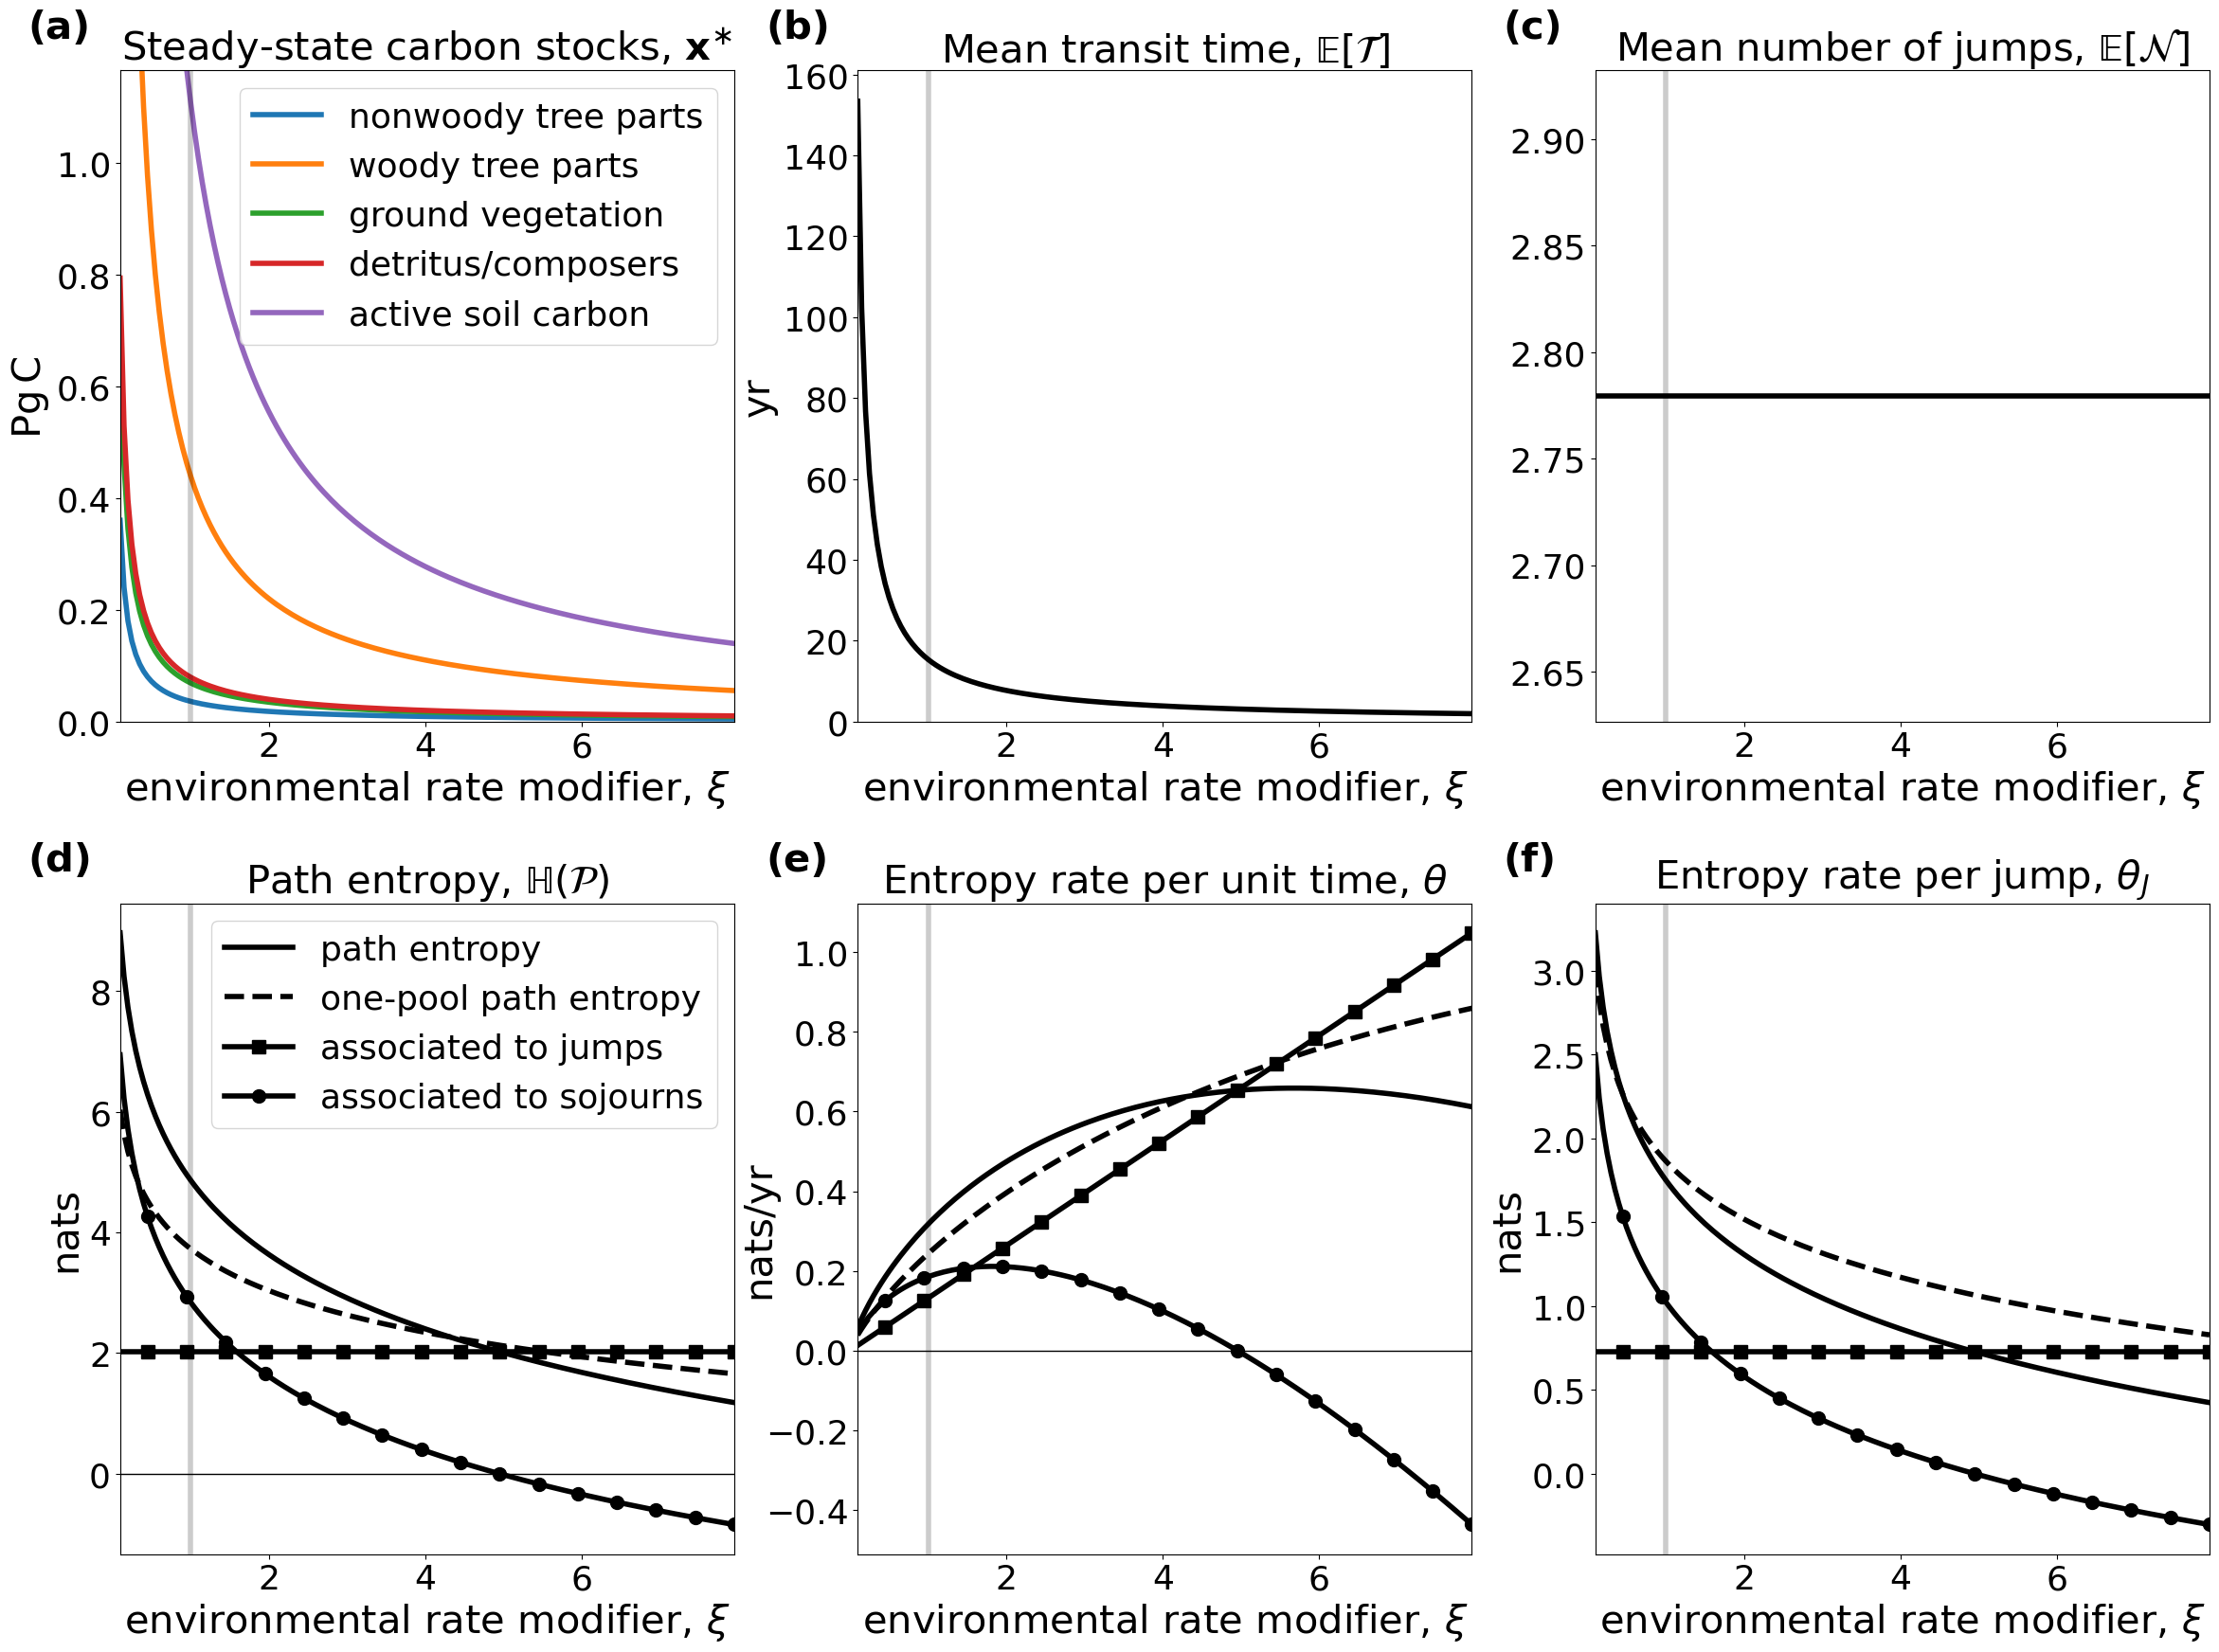
\includegraphics[width=1.0\linewidth]{figs/Emanuel_entropies.png}
    \caption{
%     A) Equilibrium carbon stocks. B)--F) Entropy related quantities of the global carbon cycle model introduced by \citet{Emanuel1981} in dependence on the environmental rate coefficient $\xi$ (solid black lines).
%     Dashed lines correspond to the quantities derived from a one-pool model with the same speed.
%     Vertical gray lines show $\xi=1$, the original speed of the model.
%     In panels D)--F) the solid lines marked by squares represent uncertainties associated to jumps (Eq.~\eqref{eqn:H_discrete}) and the solid lines marked by circles uncertainties associated to sojourn times (Eq.~\eqref{eqn:H_continuous}) such that the two marked lines sum up to the unmarked solid line.
    (a) Equilibrium carbon stocks and (b)--(f) entropy related quantities of the global carbon cycle model introduced by \citet{Emanuel1981} in dependence on the environmental rate coefficient $\xi$
  }
  \label{fig:Emanuel_entropies}
\end{figure}


\subsection{A nonlinear autonomous soil organic matter decomposition model}
\label{sec:example_2}
Consider the nonlinear two-compartment model $M_\varepsilon=M(\vec{u},\,\tens{B}_\varepsilon)$ described by \citet{Wang2014BG} which is used to represent the dynamics of microbes and carbon substrates in soils (Fig.~\ref{fig:Wang_model}). Its ODE system is given by
\begin{equation}
    \deriv{t}\,\begin{pmatrix}C_{s}\\C_{b}\end{pmatrix}(t) = 
    \begin{pmatrix}
      -\lambda(\vec{x}(t)) & \mu_{b}\\
      \varepsilon \lambda(\vec{x}(t)) & - \mu_{b}
    \end{pmatrix}
    \, \begin{pmatrix}C_{s}\\C_{b}\end{pmatrix}
    + \begin{pmatrix}F_{\NPP}\\0\end{pmatrix},
\end{equation}
where $\vec{x}(t)=(C_{s},\,C_{b})^{\transpose}(t)$.
We denote by $C_s$ and $C_b$ soil organic carbon and soil microbial biomass carbon ($\gC\,\meter^{-2}$), respectively, by $\varepsilon$ the carbon use efficiency or fraction of assimilated carbon that is converted into microbial biomass (unit-less), by $\mu_b$ the turnover rate of microbial biomass per year ($\yr^{-1}$), by $F_{\NPP}$ the carbon influx into the soil ($\gC\,\meter^{-2}\,\yr^{-1}$), and by $V_s$ and $K_s$ the maximum rate of soil carbon assimilation per unit microbial biomass per year ($\yr^{-1}$) and the half-saturation constant for soil carbon assimilation by microbial biomass ($\gC\,\meter^{-2}$), respectively.

\begin{figure}[htbp]
    \centering
    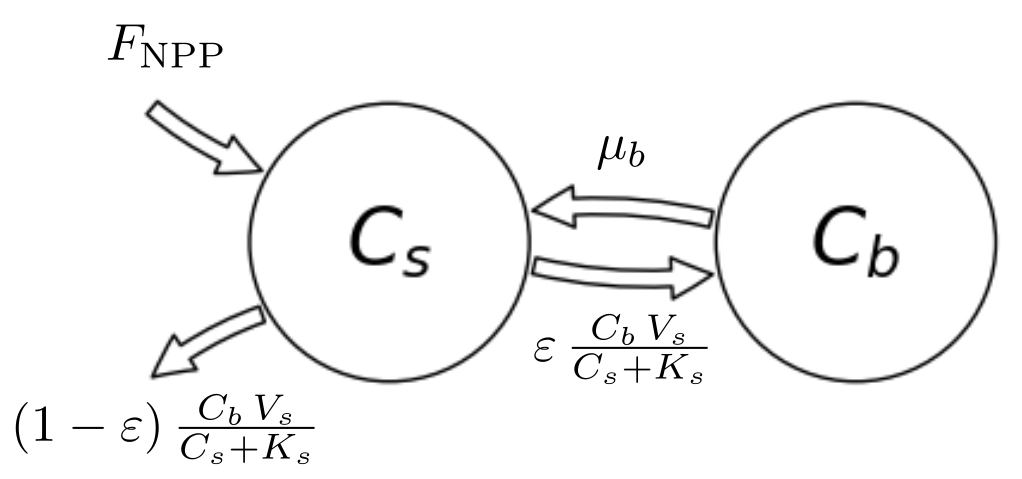
\includegraphics[width=0.5\linewidth]{figs/Wang_model_srm_with_fluxes.png}
    \caption{
%     Scheme of the nonlinear autonomous carbon cycle model introduced by \citet{Wang2014BG}. 
%     The two compartments $C_s$ and $C_b$ represent substrate organic carbon and microbial biomass carbon, respectively.
%     The external input flux is denoted by $F_{\NPP}$, the maximum rate of soil carbon assimilation by $V_s$, the half saturation constant by $K_s$, the carbon use efficiency by $\varepsilon$, and the turnover rate of microbial biomass by $\mu_b$, respectively.
    Scheme of the nonlinear autonomous carbon cycle model introduced by \citet{Wang2014BG} with two compartments: substrate organic carbon ($C_s$) and microbial biomass ($C_b$)
    }
    \label{fig:Wang_model}
\end{figure}

We consider the model in equilibrium, \ie\ $\vec{x}(t)=\vec{x}^\ast=(C_s^\ast,\,C_b^\ast)^T$ with
\begin{equation}
  C_s^\ast = \frac{K_{s}}{\frac{V_{s} \varepsilon}{\mu_{b}} - 1}\quad\text{ and }\quad C_b^\ast = \frac{F_{\NPP}}{\mu_{b} \left(-1 + \frac{1}{\varepsilon}\right)}.
\end{equation}
The equilibrium stocks depend on the carbon use efficiency $\varepsilon$ and so does the compartmental matrix $\tens{B}=\tens{B}_\varepsilon$, because
\begin{equation}\label{eqn:lambdax}
    \lambda(\vec{x}) = \frac{C_{b} V_{s}}{C_{s} + K_{s}}.
\end{equation}
From \citet{Wang2014BG} we take the parameter values $\mu_b = 4.38\,\yr^{-1}$, $F_{\NPP} = 345.00\,\gC\,\meter^{-2}\,\yr^{-1}$, and $K_s = 53,954.83\,\gC\,\meter^{-2}$.
Since the description of $V_s$ is missing in the original publication, we let it be equal to $59.13\,\yr^{-1}$ to approximately meet the given steady-state contents $C_s^\ast = 12,650.00\,\gC\,\meter^{-2}$ and $C_b^\ast = 50.36\,\gC\,\meter^{-2}$ for the original value $\varepsilon=0.39$.
Otherwise we leave the carbon use efficiency $\varepsilon$ as a free parameter.

In contrast to the system from the first example, this system exhibits a feedback.
This feedback results from dead soil microbial biomass being considered as new soil organic matter.
The feedback can also be recognized by noting that $\tens{B}$ is not triangular.
For every value of $\varepsilon$ the system has a different steady state (Fig.~\ref{fig:Wang_entropies}, panel (a)).
The higher the value of $\varepsilon$, the lower the equilibrium substrate organic carbon and the higher the microbial biomass carbon.
Caused by the model's nonlinearity expressed in Eq.~\eqref{eqn:lambdax}, the system speed increases and the mean transit time goes down (panel (b)) with increasing $\varepsilon$.
At the same time, higher carbon use efficiency increases the probability of each carbon atom to be reused more often, hence the mean number of jumps increases (panel (c)), making the entropy rate per jump decrease (panel (f)).
Even though the average paths become shorter, with increasing carbon use efficiency the path entropy increases as well for most values of $\varepsilon$.
This has two reasons.
First, the mean uncertainty of where to jump from $C_s$ increases, this uncertainty decreases then for $\varepsilon>0.5$ (solid line marked by squares in panel (f)).
Second, the rate $-B_{11}$ of leaving the substrate pool is increasing and smaller than $1$.
The corresponding Poisson process reaches its maximum entropy rate at an intensity rate equal to $1$ (Fig.~\ref{fig:simple_entropy}, panel (c)), which corresponds to $\varepsilon\approx0.926$.
This is also reflected in the entropy rate per unit time (panel (e)).
The maximum does not exactly occur at $\varepsilon=0.926$, because the times that the particle stays in the different pools also depends on $\varepsilon$.
For $\varepsilon$ approaching $1$, both the path entropy and the entropy rate rapidly decline as the sojourn-associated uncertainties (solid lines with circle markers) decline sharply because of a nonlinear increase of the rate $-B_{11}$ of soil organic carbon turnover.

Considering a one-pool system $M_\lambda=M(345.00\,\gC\,\meter^{-2}\,\yr^{-1},\, -1/\E\left[\TT_\varepsilon\right])$ with the same mean transit time, we recognize only small sensitivity of the entropies on $\varepsilon$, because the contrary effects on path length and jump- and sojourn-associated uncertainties mostly balance out (dashed lines in panels d--f).

\begin{figure}[htbp]
    \centering
    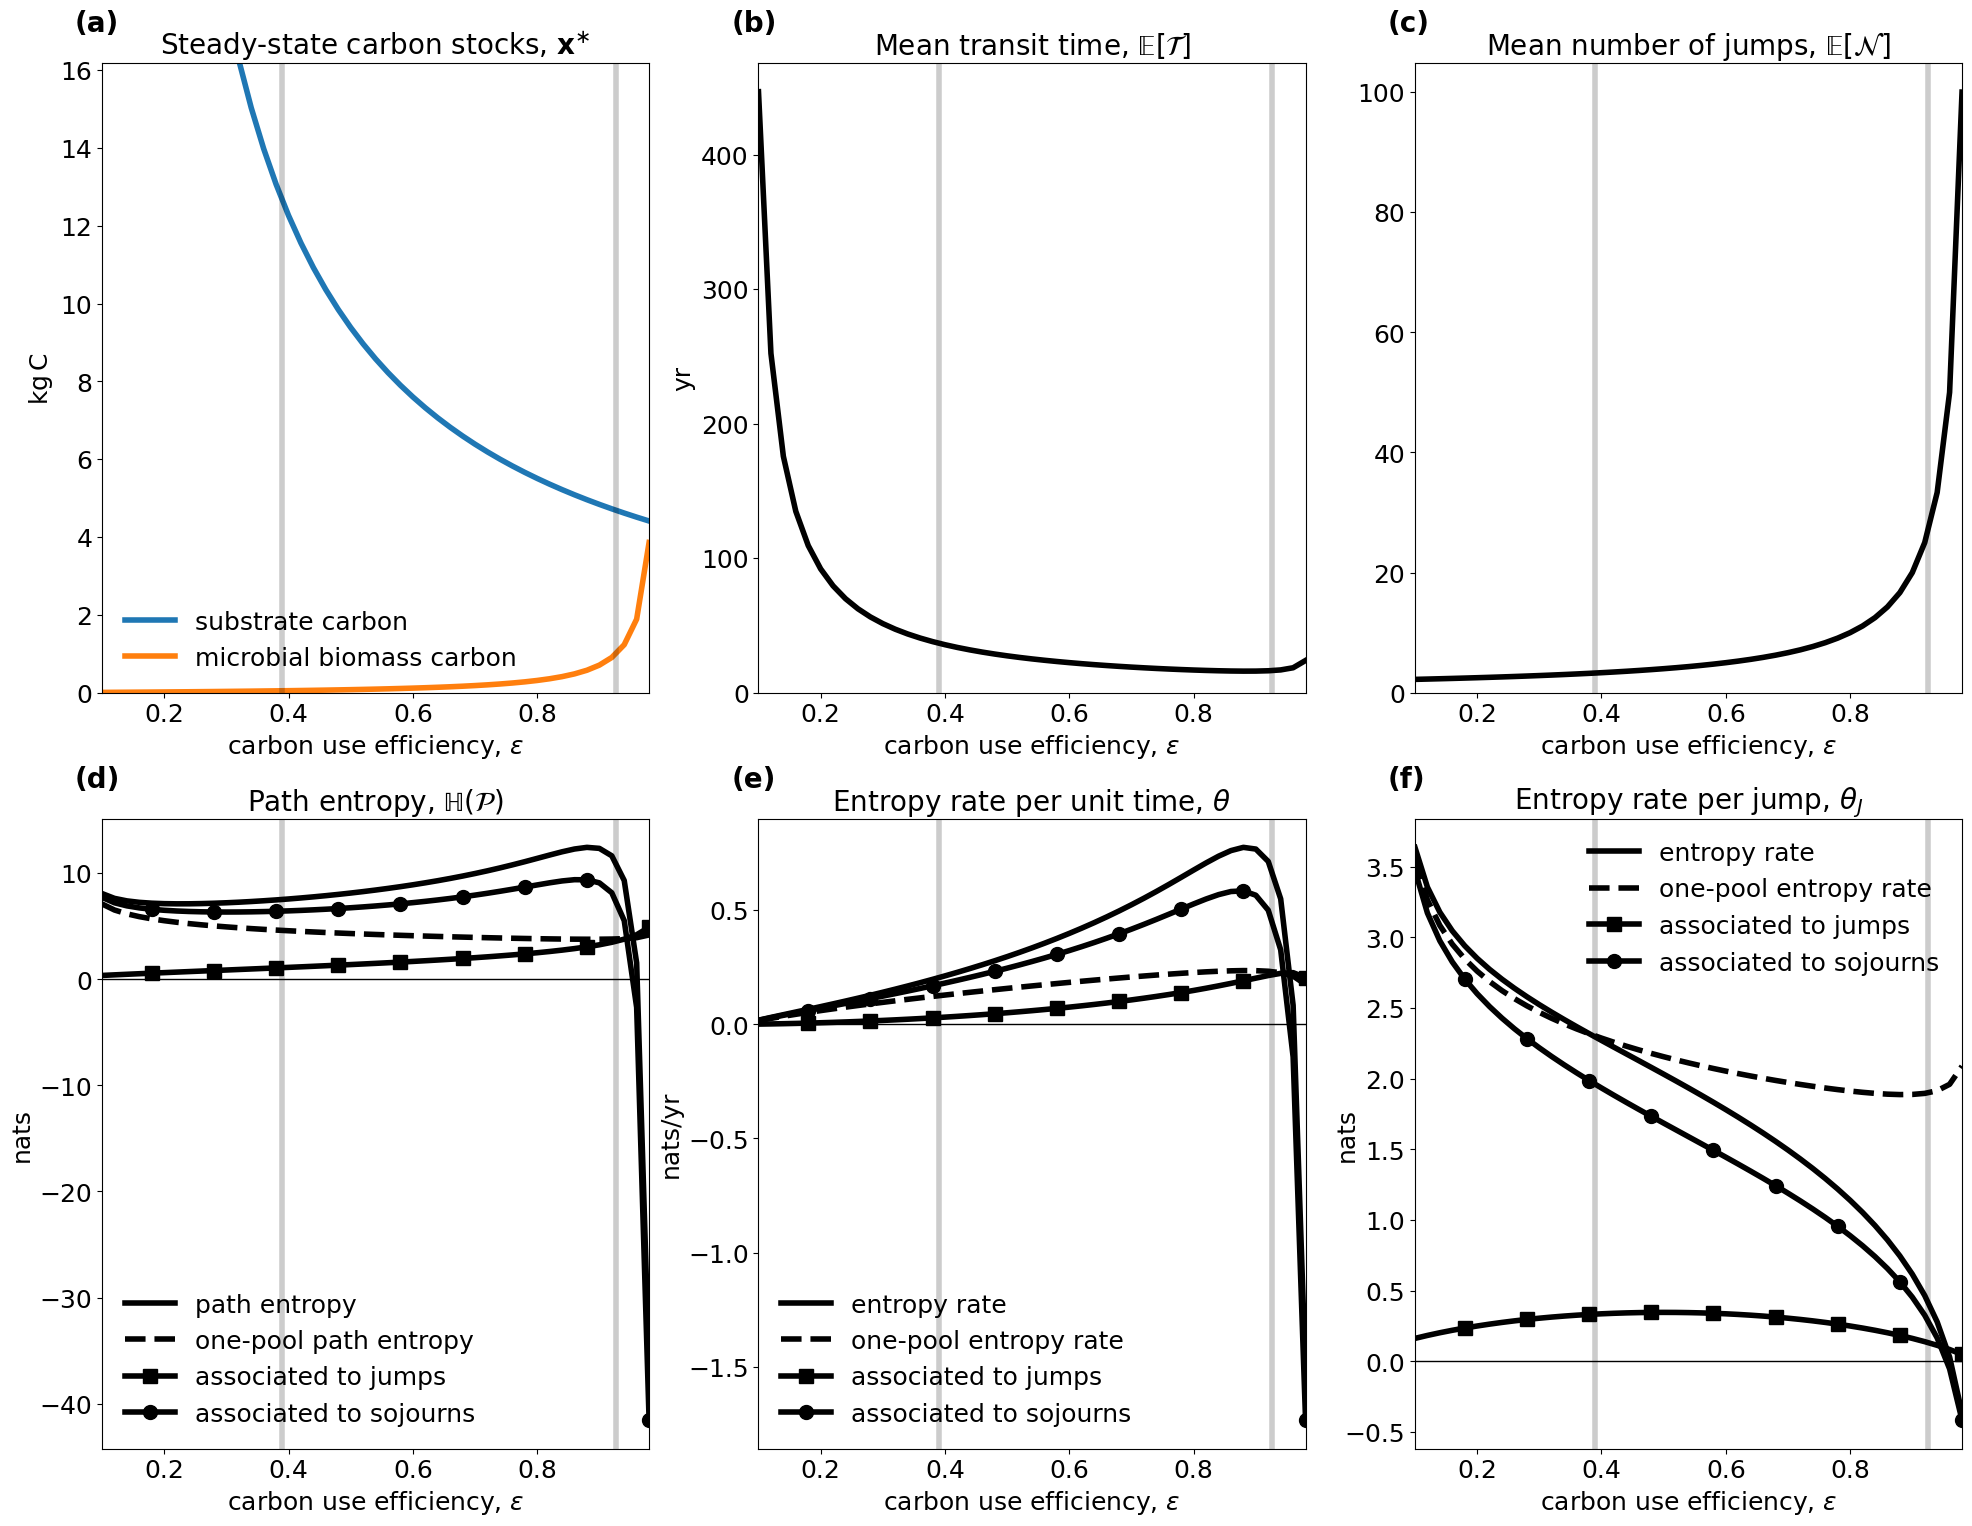
\includegraphics[width=1.0\linewidth]{figs/Wang_entropies.png}
    \caption{
    (a) Equilibrium carbon stocks and (b)--(f) entropy related quantities of the global carbon cycle model introduced by \citet{Wang2014BG} in dependence on the microbial carbon use efficiency $\varepsilon$
%     Dashed lines correspond to the quantities derived from a one-pool model with the same speed.
%     The left vertical gray lines show $\varepsilon=0.39$, the original carbon use efficiency of the model, the right ones at $\varepsilon=0.926$ show the carbon use efficiency value with the maximum entropy rate of the Poisson process associated with $C_s$.
%     In panels D)--F) the solid lines marked by squares represent uncertainties associated to jumps (Eq.~\eqref{eqn:H_discrete}) and the solid lines marked by circles uncertainties associated to sojourn times (Eq.~\eqref{eqn:H_continuous}) such that the two marked lines sum up to the unmarked solid line.    
    }
    \label{fig:Wang_entropies}
\end{figure}


\subsection{Model identification via Maxent}
  \label{sec:model_identification}
  The following example is inspired by \citet[Example~16\,C]{Anderson1983}.
  It shows how MaxEnt can help take a decision which model to use if not all parameters can be uniquely determined from the transfer function $\widehat{\tens{\Psi}}$.
	We are interested in determining the entries of the compartmental matrix $\tens{B}$ belonging to the $2$-dimensional equilibrium compartmental system
	\begin{equation}\label{eqn:opt_example}
        \deriv{t}\,
		\begin{pmatrix} x_1 \\ x_2 \end{pmatrix}(t)
		=
		\begin{pmatrix} B_{11} & B_{12} \\ B_{21} & B_{22} \end{pmatrix}\,
		\begin{pmatrix} x_1 \\ x_2 \end{pmatrix}(t)
		+
		\begin{pmatrix} 1 \\ 0 \end{pmatrix}\,\gC\,\yr^{-1},
		\quad t>0.
	\end{equation}
	We immediately notice $\vec{u}=(1,0)^T\,\gC\,\yr^{-1}$ and $\tens{A}=\tens{I}$.
	Further, we decide to measure the contents of compartment $1$ such that $\tens{C} = (1,0)$.
	We recall $z_j = -\sum_{i=1}^d B_{ij}$ and obtain $z_1 = -B_{11} - B_{21}$ and $z_2 = - B_{22} - B_{12}$.
	The real-valued transfer function is then given by
	\begin{equation}
		\widehat{\tens{\Psi}}(s) = \frac{s + \gamma_1}{s^2+\gamma_2\,s+\gamma_3},
	\end{equation}
	where
	\begin{equation}\label{eqn:measurement_data}
		\begin{aligned}
			\gamma_1 &= B_{12} + z_2,\\
			\gamma_2 &= B_{21} + z_1 + B_{12} + z_2,\\
			\gamma_3 &= z_1\,B_{12} + z_1\,z_2 + B_{21}\,z_2.
		\end{aligned}
	\end{equation}
	We assume that $\widehat{\tens{\Psi}}$ is known from measurements, \ie, $\gamma_1$, $\gamma_2$, and $\gamma_3$ are known impulse response parameters.	
	We have the four unknown parameters $B_{11}$, $B_{12}$, $B_{21}$, and $B_{22}$, or equivalently, $B_{12}$, $B_{21}$, $z_1$, and $z_2$, but only three equations to determine them.
	Consequently, the system is nonidentifiable and there remains a class $\mathcal{M}$ of models which all satisfy Eq.~\eqref{eqn:measurement_data}.
	Which model out of $\mathcal{M}$ are we going to select now?

	Here, MaxEnt comes into play.
	We intend to select the model that best represents the information given by our measurement data.
	We have to find $M^\ast=M(\vec{u},\tens{B}^\ast)$ such that
	\begin{equation}
		M^\ast = \operatornamewithlimits{arg\,max}\limits_{M\in\mathcal{M}}\,\theta(M).
	\end{equation}
	We maximize the entropy rate per unit time here instead of the path entropy, because by slowing down the model we could potentially increase its mean transit time and with it its path entropy indefinitely.
	
	Let us turn to a numerical example in which we suppose to be given $\gamma_1=3\,\yr^{-1}$, $\gamma_2=5\,\yr^{-1}$, and $\gamma_3=4\,\yr^{-1}$.
	A nonlinear optimization algorithm with the arbitrarily chosen initial values $B_{12}=3\,\yr^{-1}$, $B_{21}=0\,\yr^{-1}$, $z_1=1\,\yr^{-1}$, and $z_2=1\,\yr^{-1}$ ends approximately with the terminal compartmental matrix
	\begin{equation}
		\tens{B}^\ast \approx \begin{pmatrix} -2.00 & 1.90 \\ 1.05 & -3.00 \end{pmatrix}\,\yr^{-1}
	\end{equation}
	and the terminal entropy rate per unit time $\theta(M^\ast) \approx 1.92\,\nats\,\yr^{-1}$.
	Unfortunately, this local maximum solution it is not guaranteed to be a global maximum entropy model in $\mathcal{M}$.
	
	The nonidentifiability of the model from $\widehat{\tens{\Psi}}$ alone is underlined by the fact that another system $\widetilde{M}=M(\vec{u},\widetilde{\tens{B}})\in\mathcal{M}$ with
	\begin{equation}
		\widetilde{\tens{B}} =
		\begin{pmatrix}
			-2.00 & 2.00 \\ 1.00 & -3.00
		\end{pmatrix}
		\,\yr^{-1}
	\end{equation}
	results in the same transfer function, but a different entropy rate per unit time, \ie, $\theta(\widetilde{M}) \approx 1.90\,\nats\,\yr^{-1}$.
	Following MaxEnt, in this example we select $M^\ast$, which is found by a nonlinear optimization process whose evolution is depicted by the solid line in Fig.~\ref{fig:optimization}.
	Peaks higher than the terminal value show attempts of the optimization algorithm that do not perfectly satisfy all constraints and are rejected.
	The dashed line shows the entropy rate per unit time of model $\widetilde{M}$.

	\begin{figure}[ht]
    \centering
    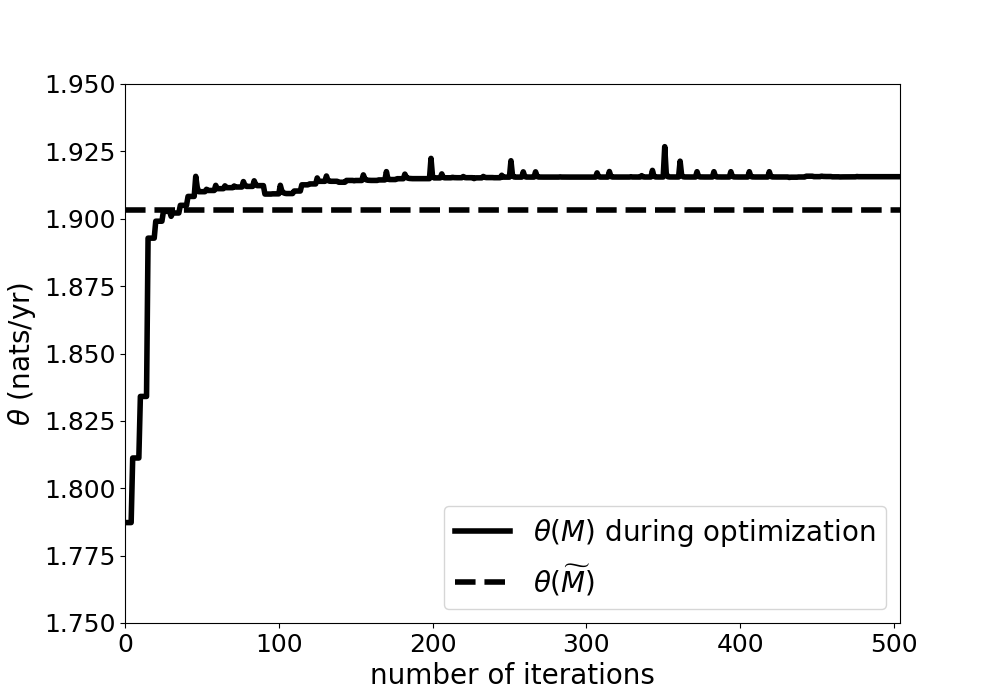
\includegraphics[width=0.95\linewidth]{figs/optimization.png}
		\caption{
% 		Entropy rate per unit time of system~\eqref{eqn:opt_example}. The solid curve shows the evolution of the entropy rate per unit time during the nonlinear optimization process.
% 		Peaks higher than the terminal value show attempts of the optimization algorithm that do not perfectly satisfy all constraints.
% 		The dashed line shows the entropy rate per unit time of model $\widetilde{M}$.
		Evolution of the entropy rate per unit time of system~\eqref{eqn:opt_example} during the nonlinear optimization process for model identification
		}
		\label{fig:optimization}
  \end{figure}



\section{Discussion}
Based on the path that a particle takes through a compartmental system, we introduced three types of entropy based on Shannon's information theory.
The entropy of the particle's entire path through the system is the central concept, and the entropy rates per unit time and per jump are consistently derived from it.
Even though we call $\H(\mathcal{P})$ path entropy and identify models by maximizing it, it is different from the concept of path entropy as treated in the context of maximum caliber (MaxCal) \citep{jaynes1985macroscopic}.
We maximize here the Shannon entropy of a single particle's microscopic path through a compartmental system by means of an absorbing continuous-time Markov chain whose transition probabilities are already determined by the macroscopic equilibrium state of the system.
As discussed by \citet{Presse2013RMP}, MaxCal interprets the path entropy as a macroscopic system property to be maximized in order to identify a time-dependent trajectory of the entire dynamical system, not just one single particle.

In the field of soil carbon cycle modeling, \citet{Agren2021BGC} recently applied the maximum entropy principle to identify the distribution of soil carbon qualities within the framework of the continuous-quality theory.
Given only the nonnegative mean quality, an application of MaxEnt leads to an exponential quality distribution, because under these circumstances the exponential distribution is the maximum entropy distribution.
The path entropy generalizes this approach to several interconnected compartments and jumps between them, while each sojourn time in a compartment is exponentially distributed.

From the simple examples in Sect.~\ref{sec:simple_examples} we can see that models can be ordered differently in terms of uncertainty, depending on whether the interest is in the uncertainty of the entire path or in some average uncertainty rate.
For applications of MaxEnt without restrictions on the transit time, it is often useful to maximize an entropy rate because by slowing the system down more and more, the path entropy can potentially be increased indefinitely and there is no way to find a maximum path entropy model.

Usually, entropy is maximized when the system is highly symmetric.
This is indicated by the Bernoulli entropy (Fig.~\ref{fig:simple_entropy}, panel (a)) and supported by Example~\ref{max_ent_example_1}.
Intuitively, this result is obvious.
If a system has high symmetry, a particle is equally likely to jump among different pools, and the Poisson process with intensity rate $1$ is the one with maximum entropy rate.
Furthermore, the resulting rates $z_j = 1/\E\left[\TT\right]$ of leaving the system are chosen such that the mean transit time constraint is fulfilled. 
In Example~\ref{max_ent_example_2}, the symmetry is broken by the additional restriction of a given steady-state vector.
Consequently, $\H(M_2) \leq \H(M_1)$.

When we compute entropy values for actual carbon-cycle models (Sects.~\ref{sec:example_1} and~\ref{sec:example_2}), we note that environmental or biochemical factors impact the model entropies.
Furthermore, we see that for sufficiently fast systems, a multi-pool model has lower entropy than a one-pool model with the same system speed.
The one-pool system might put too much weight on the uncertainties of a small amount of slow-cycling particles, while the more detailed multi-pool model focuses more on the small uncertainties of the major amount of fast-cycling particles.
The path of a detailed model that separates fast from slow paths is then even easier to predict than a one-pool model path, even though the detailed model's path looks more complicated.
However, detailed paths of slow-cycling systems are harder to predict than just the exit-time in a one-pool equivalent.

The example of model identification by MaxEnt in Sect.~\ref{sec:model_identification} shows a major difference to the more artificial previous maximum entropy examples.
The given constraints do not tell us enough about the structure of the model class $\mathcal{M}$ to ensure that an identified local maximum is also a global maximum.
It might be possible that with different initial values the optimization algorithm finds another local maximum model with higher entropy rate.
This example is only supposed to give a first impression of how the maximum entropy principle can be used in combination with entropy rates or path entropy in similar situations.
Practical examples usually have a high level of complexity such that existence and uniqueness of a maximum entropy model have to be studied on a case-by-case basis.


\section{Conclusions}
Information content and complexity of autonomous compartmental systems in equilibrium can be assessed by the entropy of the path of particles traveling through a system of interconnected compartments. When a particle moves through a compartmental system, it creates a path from the time of its entry until the time of its exit. This path can be described in three ways: (1) as a random variable in the path space; (2) as a continuous-time stochastic process representing the visited compartments; (3) as a discrete sequence of pairs consisting of visited compartments and associated sojourn times. 
Based on these three ways, we introduced for systems in equilibrium (1) the entropy of the entire path, (2) the entropy rate per unit time, and (3) the entropy rate per jump. These three different entropies allow to quantify how difficult it is to predict the path of particles entering a compartmental system, serving as a measure of complexity and information content. With these measures, it is thus possible to apply maximum entropy principles to compartmental systems in equilibrium in order to address problems of equifinality in model selection. 

Although the path entropy concept developed here only applies to systems in equilibrium, it sets the foundation for future research on systems out of equilibrium. 
This could be done by building on the concept of the entropy rate per unit time as an instantaneous uncertainty and interpreting non-autonomous compartmental systems as inhomogeneous Markov chains.
This would allow an extension of MaxCal applied only to the inhomogeneous embedded jump chain as done by \citet{Ge2012JCP}.

By introducing the concept of path entropy to compartmental systems, we made a first crucial step toward a quantification of information content in models that can be compared to other methods to obtain information content from observations. Using entropy measures in both models and observations, we could potentially advance toward better methods for model selection applying the maximum entropy principle. 

\newpage

\begin{acknowledgements}
Funding was provided by the Max Planck Society and the German Research Foundation through its Emmy Noether Program (SI 1953/2--1) and the Swedish Research Council for Sustainable Development FORMAS, under grant 2018-01820.
\end{acknowledgements}

% \bibliographystyle{spbasic}
\bibliographystyle{MG}
{footnotesize
\bibliography{entropy.bib}}


\appendix

\section{Basic ideas of Shannon information entropy}
\label{sec:entropy_basics_extended}
We introduce basic concepts of information entropy along the lines of \citet{Cover2006}.
There are two concepts of entropy of a random variable, depending on whether the random variable has a discrete or a continuous distribution.
\begin{definition}%[Entropy]
\label{def:discrete_entropy}
	(1) Let $Y_d$ be a discrete real-valued random variable with range $R_d$ and probability mass function $p$.
	The \emph{Shannon information entropy} or \emph{Shannon entropy} or \emph{information entropy}, or simply \emph{entropy} of $Y_d$ is defined by
	\begin{equation}
		\H(Y_d) = -\suml_{y\in R_d} p(y)\,\log p(y) = -\E\left[\log p(Y_d)\right].
	\end{equation}
	By convention, $0\,\log 0:=0$.
	
	(2) Let $Y_c$ be a continuous real-valued random variable with range $R_c$ and \pdf\ $f$.
	Then the \emph{differential entropy} or simply \emph{entropy} of $Y_c$ is defined by
	\begin{equation}
		\H(Y_c) = -\intl_{R_c} f(y)\,\log f(y)\dd{y} = -\E\left[\log f(Y_c)\right].
	\end{equation}
\end{definition}

\begin{myremark}
	Depending on the base of the logarithm, the unit of the entropy changes.
	For base $2$, the unit is called \emph{$\bits$} and for the natural logarithm with base $e$, the unit is called \emph{$\nats$}.
	If not stated differently, we use the value $e$ as logarithmic base, \ie, we use the natural logarithm.
\end{myremark}

The entropy $\H(Y)$ of a random variable $Y$ has two intertwined interpretations.
On the one hand, $\H(Y)$ is a measure of uncertainty, \ie, a measure of how difficult it is to predict the outcome of a realization of $Y$.
On the other hand, $\H(Y)$ is also a measure of the information content of $Y$, \ie, a measure of how much information we gain once we learn about the outcome of a realization of $Y$.
It is important to note that, even though their definitions and information theoretical interpretations are quite similar, the Shannon- and the differential entropy are of different nature.
The Shannon entropy is always nonnegative, whereas the differential entropy can have negative values.
Consequently, the Shannon entropy is an absolute measure of information and makes sense in its own right.
The differential entropy, however, is not an absolute information measure.
Hence, the differential entropy of a random variable makes sense only in comparison with the differential entropy of another random variable.

Panel (a) of Fig.~\ref{fig:simple_entropy} depicts the Shannon entropy of a Bernoulli random variable $Y_d$ with $\P(Y_d=1)=1-\P(Y_d=0)=p\in[0,1]$.
This random variable could represent the outcome of a coin toss.
We can see that the entropy is low when $p$ is close to $0$ or $1$.
In these cases, we have some information that the coin is biased, and hence we have a preference if we guess the outcome.
The entropy is maximum if the coin is fair ($p=1/2$), since we have no additional information about the outcome of the coin toss.
The Shannon entropy of $Y_d$ is
\begin{equation}
	\H(Y_d) = -p\,\log p - (1-p)\,\log(1-p).
\end{equation}

Panel (b) of Fig.~\ref{fig:simple_entropy} shows the differential entropy of an exponentially distributed random variable $Y_c\sim\Exp(\lambda)$ with rate parameter $\lambda>0$, \pdf\ $f(y) = \lambda\,e^{-\lambda\,y}$ for $y\geq0$, and $\E\left[Y_c\right]=\lambda^{-1}$.
We can imagine it to represent the duration of stay of a particle in a well-mixed compartment in a linear autonomous compartmental system, where $\lambda$ is the total outflow rate from the compartment.
The higher the outflow rate, the likelier an early exit of the particle, and the easier it is to predict the moment of exit.
Hence, the differential entropy
\begin{equation}
	\H(Y_c) = 1-\log\lambda
\end{equation}
decreases with increasing $\lambda$.

\begin{definition}%[Joint entropy]
		Let $Y_1,Y_2$ be two discrete random variables with joint probability mass function $p$ and ranges $R_1$ and $R_2$, respectively.
		The \emph{joint entropy} of $Y_1$ and $Y_2$ is defined by
		\begin{equation}
			\H(Y_1,Y_2) = -\suml_{y_1\in R_1}\suml_{y_2\in R_2} p(y_1,y_2)\,\log p(y_1,y_2) = -\E\left[\log p(Y_1,Y_2)\right].
		\end{equation}
\end{definition}
Note that the joint entropy is symmetric, \ie, $\H(Y_1,Y_2) = \H(Y_2,Y_1)$.
Furthermore, $\H(Y_1,Y_2)\leq \H(Y_1) + \H(Y_2)$ with equality if $Y_1$ and $Y_2$ are independent.

\begin{definition}%[Conditional entropy]
\label{def:conditional_entropy}
	Let $Y_1$ and $Y_2$ be two discrete random variables with joint probability mass function $p$.
	Furthermore, let $p_2$ denote the probability mass function of $Y_2$ and denote by $p(y_1\,|\,y_2)$ the conditional probability $\P(Y_1=y_1\,|\,Y_2=y_2)$.
	
	Then the \emph{conditional entropy} of $Y_1$ given $Y_2$ is defined by
	\begin{equation}
		\begin{aligned}
			\H(Y_1\,|\,Y_2) &= \suml_{y_2\in R_2} \H(Y_1\,|\,Y_2=y_2)\,p_2(y_2)\\
			&= -\suml_{y_2\in R_2} p_2(y_2)\suml_{y_1\in R_1}p(y_1\,|\,y_2)\,\log p(y_1\,|\,y_2)\\
			&= -\suml_{y_2\in R_2}\suml_{y_1\in R_1} p(y_1,y_2)\,\log p(y_1\,|\,y_2)\\
			&= -\E\left[\log p(Y_1\,|\,Y_2)\right].
		\end{aligned}
	\end{equation}
\end{definition}
Note that $\H(Y_1\,|\,Y_2)\leq \H(Y_1)$ with equality if $Y_1$ and $Y_2$ are independent.
The joint entropy of two random variables is the entropy of one variable plus the conditional entropy of the other.
This is expressed in 
\begin{equation}\label{eqn:two_expansion_rule}
	\H(Y_1,Y_2) = \H(Y_2) + \H(Y_1\,|\,Y_2).
\end{equation}
Let $Y_3$ be a third discrete random variable.
Then
\begin{equation}\label{eqn:three_expansion_rule}
	\H(Y_1,Y_2\,|\,Y_3) = \H(Y_1\,|\,Y_3) + \H(Y_2\,|\,Y_1,Y_3).
\end{equation}
Let $Y_1,Y_2,\ldots,Y_n$ be discrete random variables.
By repeated application of Eq.~\eqref{eqn:two_expansion_rule} and Eq.~\eqref{eqn:three_expansion_rule}, we obtain the \emph{chain rule}
\begin{equation}\label{eqn:chain_rule}
	\H(Y_1,Y_2,\ldots,Y_n) = \suml_{k=1}^n \H(Y_k\,|\,Y_{k-1},\ldots,Y_1).
\end{equation}

\begin{myremark}
	We defined the joint- and conditional entropy for discrete random variables only.
	Analogous definitions can be made for continuous random variables.
	Also the chain rule holds for differential entropy.
\end{myremark}

\begin{definition}%[Discrete-time entropy rate]
\label{def:entropy_rate}
	The \emph{entropy rate} of a discrete-time stochastic process $Y=(Y_n)_{n\in \N}$ is defined by
	\begin{equation}
		\theta(Y) = \liml_{n\to\infty} \frac{1}{n}\,\H(Y_1,Y_2,\ldots,Y_n) = -\frac{1}{n}\,\E\left[\log p_n(Y_1,Y_2,\ldots,Y_n)\right]
	\end{equation}
	if the limit exists.
	Here, $p_n$ denotes the joint probability mass function of $Y_1,Y_2,\ldots,Y_n$.
\end{definition}

The discrete-time entropy rate describes the long-term average increase of the processes' entropy per time step.
The statements of the following lemma are proven in \citet[Theorem~4.2.1]{Cover2006}.

\begin{mylemma}\label{lem:entropy_rate_st_MC}
	For a stationary discrete-time stochastic process $Y=(Y_n)_{n\in\N}$, the entropy rate is
	\begin{equation}
		\theta(Y) = \liml_{n\to\infty} \H(Y_n\,|\,Y_{n-1},\ldots,Y_1).
	\end{equation}
	Consequently, if $Y$ is a stationary discrete-time Markov chain, its entropy rate is
	\begin{equation}
		\theta(Y) = \H(Y_2\,|\,Y_1).
	\end{equation}
\end{mylemma}

According to \citet{Dumitrescu1988MICAS} and \citet{Girardin2003JAP}, we can also define the entropy rate for continuous-time processes.
To that end, we first define the entropy on a finite time interval.

\begin{definition}%[Finite-time entropy]
	The \emph{finite-time entropy} of the continuous-time stochastic process $Z=(Z_t)_{t\geq0}$ until $T\geq0$ is defined as
	\begin{equation}
		\H_T(Z) = - \int f_T(z)\,\log f_T(z)\dd{\mu_T(z)},	 
	\end{equation}
	where $f_T$ is the \pdf\ of $(Z_t)_{0\leq t\leq T}$ with respect to some reference measure $\mu_T$, if it exists.
\end{definition}

\begin{definition}%[Continuous-time entropy rate]
	The \emph{entropy rate} of a continuous-time stochastic process $Z=(Z_t)_{t\geq0}$ is defined by
	\begin{equation}
		\theta(Z) = \liml_{T\to\infty} \frac{1}{T}\,\H_T(Z)
	\end{equation}
	if the limit exists.
\end{definition}


\section{Proves of the MaxEnt examples}
	Recall that the path entropy of a linear autonomous compartmental system $M=M(\vec{u},\tens{B})$ is given by
	\begin{equation}
    \begin{aligned}
      \H(M) &= \H(X)\\
      &= -\suml_{i=1}^d\beta_i\,\log\beta_i + \suml_{j=1}^d \frac{x^\ast_j}{\vnorms{\vec{u}}}\left[\suml_{i=1,i\neq j}^d \,B_{ij}\,(1-\log B_{ij}) + z_j\,(1-\log z_j)\right].
    \end{aligned}
	\end{equation}
	In order to obtain maximum entropy models under simple constraints, we now adapt ideas of \cite{Girardin2004MCAP}.

	\begin{myproposition}
    \label{proposition:max_ent_example_1}
		Consider the set $\mathcal{M}_1$ of compartmental systems in equilibrium given by Eq.~\eqref{eqn:lin_CS_sys}  with a predefined nonzero input vector $\vec{u}$, a predefined mean transit time $\E\left[\TT\right]$, and an unknown steady-state vector comprising nonzero components.
		The compartmental system $M^\ast_1=M(\vec{u},\tens{B}^\ast)$ with 
		\begin{equation}
			\tens{B}^\ast = \begin{pmatrix}
									-\lambda & 1 & \cdots & 1\\
									1 & -\lambda & 1 \cdots & 1 \\
									\vdots & & \ddots & \vdots\\
									1 & \cdots & 1 & -\lambda
             \end{pmatrix},
		\end{equation}
		where $\lambda=d-1+1/\E\left[\TT\right]$, 		
		is the maximum entropy model in $\mathcal{M}_1$.
	\end{myproposition}

	\begin{proof}%[Proof of Proposition~\ref{proposition:first_max_entropy_model}]
		We can express the constraint $\E\left[\TT\right] =\vnorms{\vec{x}^\ast}/\vnorms{\vec{u}}$ by
		\begin{equation}
		C_1 = \frac{1}{\vnorms{\vec{u}}}\,\suml_{j=1}^d x_j^\ast - \E\left[\TT\right] = 0.
		\end{equation}
		From the steady-state formula $\vec{x}^\ast = -\tens{B}^{-1}\,\vec{u}$, we obtain another set of $d$ constraints, which we can describe by
		\begin{equation}
			\frac{1}{\vnorms{\vec{u}}}\,(\tens{B}\,\vec{x}^\ast)_i=-\beta_i,\quad i=1,2,\ldots,d.
		\end{equation}
		We rewrite the left hand side as
		\begin{equation}
      \begin{aligned}
        \frac{1}{\vnorms{\vec{u}}}\,(\tens{B}\,\vec{x}^\ast)_i &= \frac{1}{\vnorms{\vec{u}}}\,\suml_{j=1}^d B_{ij}\,x_j^\ast = \frac{1}{\vnorms{\vec{u}}}\,\left(\suml_{j=1,j\neq i}^d B_{ij}\,x_j^\ast + B_{ii}\,x_i^\ast\right)\\
        &= \frac{1}{\vnorms{\vec{u}}}\,\suml_{j=1,j\neq i}^d B_{ij}\,x_j^\ast-\frac{1}{\vnorms{\vec{u}}}\,x_i^\ast\,\left(\suml_{k=1,k\neq i}^d B_{ki} + z_i\right), 
      \end{aligned}
    \end{equation}
		which leads to the constraints
		\begin{equation}\label{eqn:constraint_C2}
			C_{2,i} = \frac{1}{\vnorms{\vec{u}}}\,\suml_{j=1,j\neq i}^d B_{ij}\,x_j^\ast-\frac{1}{\vnorms{\vec{u}}}\,x_i^\ast\,\left(\suml_{k=1,k\neq i}^d B_{ki} + z_i\right) + \beta_i = 0,\quad i\in S.
		\end{equation}	
		The Lagrangian is now given by
		\begin{equation}\label{eqn:Lagrangian}
			L = \H(X) + \gamma_0\,C_1 + \suml_{i=1}^d \gamma_i\,C_{2,i}
		\end{equation}
		and its partial derivatives with respect to $B_{ij}\,(i\neq j)$, $z_j$, and $ x_j^\ast$ by
    \begin{equation}
      \begin{aligned}
        \vnorms{\vec{u}}\,\pderiv{B_{ij}}\,L &=  -x_j^\ast\,\log B_{ij} +   \gamma_i\,x_j^\ast- \gamma_j\,x_j^\ast,\\
        \vnorms{\vec{u}}\,\pderiv{z_j}\,L &= -x_j^\ast\,\log z_j-\gamma_j\,x_j^\ast,
      \end{aligned}
    \end{equation}
		and
		\begin{equation}
      \begin{aligned}
        \vnorms{\vec{u}}\,\pderiv{x_j^\ast}\,L &= \suml_{i=1,i\neq j}^d B_{ij}\,(1-\log B_{ij}) + z_j\,(1-\log z_j)\\
        &\quad+ \gamma_0 + \suml_{i=1,i\neq j}^d \gamma_i\,B_{ij} - \gamma_j\,\left(\suml_{k=1,k\neq j}^d B_{kj} + z_j\right), 
      \end{aligned}
    \end{equation}
		respectively.
		Setting $\pderiv{B_{ij}}\,L=0$ gives $B_{ij} = e^{\gamma_i-\gamma_j}$, and setting $\pderiv{z_j}\,L = 0$ gives $z_j = e^{-\gamma_j}$.
		We plug this into $\pderiv{x_j^\ast}\,L=0$ and get
		\begin{equation}
      \begin{aligned}
        0 &= \suml_{i=1,i\neq j}^d e^{\gamma_i-\gamma_j}\,[1-(\gamma_i-\gamma_j)] + e^{-\gamma_j}\,[1-(-\gamma_j)]\\
        &\quad + \gamma_0 + \suml_{i=1,i\neq j}^d \gamma_i\,e^{\gamma_i-\gamma_j} - \gamma_j\,\left(\suml_{k=1,k\neq j}^d e^{\gamma_k-\gamma_j}+e^{-\gamma_j}\right)\\
        &= \suml_{i\neq j,i\neq j} e^{\gamma_i-\gamma_j}+e^{-\gamma_j} + \gamma_0.
      \end{aligned}
    \end{equation}
		Subtracting $e^{-\gamma_j}$ from both sides and multiplying with $e^{\gamma_j}$ leads to
		\begin{equation}
			\gamma_0\,e^{\gamma_j}+\suml_{i=1,i\neq j}^d e^{\gamma_i} = -1,\quad j=1,2,\ldots,d.
		\end{equation}
		This is equivalent to the linear system $\tens{Y}\,\vec{v} = \vec{-1}$ with
		\begin{equation}
			\tens{Y} = \begin{pmatrix}
									\gamma_0 & 1 & \cdots & 1\\
									1 & \gamma_0 & 1 \cdots & 1 \\
									\vdots & & \ddots & \vdots\\
									1 & \cdots & 1 & \gamma_0
								\end{pmatrix},\quad
			\vec{v} = \begin{pmatrix} e^{\gamma_1}\\ e^{\gamma_2}\\ \vdots \\ e^{\gamma_d} \end{pmatrix},\quad
			\vec{-1} = \begin{pmatrix} -1 \\ -1 \\ \vdots \\ -1 \end{pmatrix}.
		\end{equation}
		The case $\gamma_0=1$ has no solution $\vec{v}$ since $e^{\gamma_i}>0>-1$.
		For $\gamma_0\neq 1$ the matrix $\tens{Y}$ has a nonzero determinant which makes the system uniquely solvable.
		For symmetry reasons, $\gamma_i=\gamma_j=:\gamma$ for all $i,j=1,2,\ldots,d$.
		Consequently, for $i\neq j$, we get $B_{ij}=1$, and by summing Eq.~\eqref{eqn:constraint_C2} over $i\in S$,
		\begin{equation}
		\begin{aligned}
			0 &= \vnorms{\vec{u}}\,\suml_{i=1}^d C_{2,i} = \suml_{i=1}^d \suml_{j=1,j\neq i}^d B_{ij}\,x_j^\ast - \suml_{i=1}^d x_i^\ast\,\left(\suml_{k=1,k\neq i}^d B_{ki}+z_i\right) - \vnorms{\vec{u}}\\
			&= -\suml_{i=1}^d x_i^\ast\,z_i - \vnorms{\vec{u}},		
		\end{aligned}
		\end{equation}
		which can also be expressed by $\vec{z}^T\,\vec{x}^\ast = \vnorms{\vec{u}}$.
		We simply plug in $z_i=e^{-\gamma}$ and get $e^{-\gamma}\,\vnorms{\vec{x}^\ast} = \|\vec{u}\|$, which means $z_i = 1/\E\left[\TT\right]$.
		Consequently,
		\begin{equation}
			\tens{B}^\ast = \begin{pmatrix}
									-\lambda & 1 & \cdots & 1\\
									1 & -\lambda & 1 \cdots & 1 \\
									\vdots & & \ddots & \vdots\\
									1 & \cdots & 1 & -\lambda
							\end{pmatrix}
		\end{equation}
		for $\lambda=d-1+1/\E\left[\TT\right]$.
		Since uniqueness of this solution follows from its construction, we remain with showing maximality.
		To this end, we split the entropy into to three parts, \ie, $\H(X) = H_1 + H_2 + H_3$ with
		\begin{equation}
			\begin{aligned}
				H_1 &= -\suml_{i=1}^d\beta_i\,\log\beta_i,\\
				H_2 &= \suml_{j=1}^d \frac{x^\ast_j}{\vnorms{\vec{u}}}\,z_j\,(1-\log z_j), \text{ and}\\
				H_3 &= \suml_{j=1}^d \frac{x^\ast_j}{\vnorms{\vec{u}}}\,\suml_{i=1,i\neq j}^d \,B_{ij}\,(1-\log B_{ij}).
			\end{aligned}
		\end{equation}
		The term $H_1$ is independent of $B_{ij}$ and $z_j$ for all $i,j\in S$ and $i\neq j$, and can thus be ignored.
		We denote by $E$ the pool from which the particle exits from the system.
		Then we can use \citep[Sect.~5.3]{Metzler2018MGS}
		\begin{equation}
		  \P(E=j) = \frac{z_j\,x^\ast_j}{\vnorms{\vec{u}}}
		\end{equation}
    to rewrite the second term as
		\begin{equation}
			H_2 = \suml_{j=1}^d \P(E=j)\,(1-\log z_j) = \suml_{j=1}^d \H(T_E\,|\,E=j)\,\P(E=j) = \H(T_E\,|\,E),
		\end{equation}
		where $T_E$ denotes the exponentially distributed sojourn time in $E$ right before absorption.
		We see that $H_2$ becomes maximal if the knowledge of $E$ contains no information about $T_E$.
		Hence, $z_j=z_i$ for $i,j\in S$.
		Since we need to ensure the systems' constraint on $\E\left[\TT\right]$, we get $z_j=1/\E\left[\TT\right]$ for all $j\in S$.
		
		In order to see that $B_{ij}=1$ ($i\neq j$) leads to maximal entropy, we first note that 
		\begin{equation}
			H_3 = \suml_{j=1}^d \frac{x^\ast_j}{\vnorms{\vec{u}}}\,\suml_{i=1,i\neq j}^d \,1\cdot(1-\log 1) = (d-1)\,\suml_{j=1}^d \E\left[O_j\right] = (d-1)\,\E\left[\TT\right]
		\end{equation}
		by Eq.~\eqref{eqn:H_occupation_time}.
		We now disturb $B_{kl}$ for fixed $k,l\in S$ with $k\neq l$ by a sufficiently tiny $\varepsilon$, which may be positive or negative.
		We define $B_{kl}(\varepsilon):=B_{kl}+\varepsilon$, and a change from $\lambda_j$ to $\lambda_j(\varepsilon):=\lambda_j+\varepsilon>0$ ensures $z_j(\varepsilon) = z_j$, implying that the system's mean transit time remains unchanged, \ie, $\E\left[\TT(\varepsilon)\right] = \E\left[\TT\right]$.
		The $\varepsilon$-disturbed $H_3$ is given by
		\begin{equation}
      \begin{aligned}
        H_3(\varepsilon) &= \suml_{j=1}^d \frac{x^\ast_j(\varepsilon)}{\vnorms{\vec{u}}}\,\suml_{i=1,i\neq j}^d \,1\cdot(1-\log 1)\,\left(1-\mathbbm{1}_{\{i=k,\,j=l\}}\right)\\
        &\quad + \frac{x^\ast_l(\varepsilon)}{\vnorms{\vec{u}}}\,(1+\varepsilon)\,[1-\log(1+\varepsilon)]\\
        &= \suml_{j=1}^d \frac{x^\ast_j(\varepsilon)}{\vnorms{\vec{u}}}\,\suml_{i=1,i\neq j}^d \,\left(1-\mathbbm{1}_{\{i=k,\,j=l\}}\right) + \frac{x^\ast_l(\varepsilon)}{\vnorms{\vec{u}}}\,(1-\delta)\\
      \end{aligned}
    \end{equation}
		for some $\delta>0$ since the map $x\mapsto x\,(1-\log x)$ has its global maximum at $x=1$.
		Consequently,
		\begin{equation}
		\begin{aligned}
			&H_3(\varepsilon) &&= \left[\suml_{j=1}^d \frac{x^\ast_j(\varepsilon)}{\vnorms{\vec{u}}}\,\suml_{i=1,i\neq j}^d \,1\right] - \delta\,\frac{x^\ast_l(\varepsilon)}{\vnorms{\vec{u}}}
			&&= (d-1)\,\suml_{j=1}^d \E\left[O_j(\varepsilon)\right] - \delta\,\frac{x^\ast_l(\varepsilon)}{\vnorms{\vec{u}}}\\
			& &&= (d-1)\,\E\left[\TT(\varepsilon)\right] - \delta\,\frac{x^\ast_l(\varepsilon)}{\vnorms{\vec{u}}}
			&&= (d-1)\,\E\left[\TT\right] - \delta\,\frac{x^\ast_l(\varepsilon)}{\vnorms{\vec{u}}}\\
			& && < H_3.
		\end{aligned}
	\end{equation}
		Hence, disturbing $B_{ij}$ away from $1$ reduces the entropy of the system, and the proof is complete.
	\end{proof}
	
	\begin{myproposition}
    \label{proposition:max_ent_example_2}
		Consider the set $\mathcal{M}_2$ of compartmental systems in equilibrium given by Eq.~\eqref{eqn:lin_CS_sys} with a predefined nonzero input vector $\vec{u}$ and a predefined positive steady-state vector $\vec{x}^\ast$.
		The compartmental system $M^\ast_2=M(\vec{u},\tens{B}^\ast)$ with $\tens{B}^\ast=(B_{ij})_{i,j\in S}$ given by
		\begin{equation}
			B_{ij} = \begin{cases}
							\sqrt\frac{x_i^\ast}{x_j^\ast},\quad & i\neq j,\\
							-\suml_{k=1,k\neq j}^d \sqrt\frac{x_k^\ast}{x_j^\ast} - \frac{1}{\sqrt{x_j^\ast}}, \quad &i=j,
						\end{cases}
		\end{equation}
		is the maximum entropy model in $\mathcal{M}_2$.
	\end{myproposition}

	\begin{proof}
		The mean transit time $\E\left[\TT\right]=\vnorms{\vec{x}^\ast}/\vnorms{\vec{u}}$ of the system is fixed.
		Hence, the Lagrangian $L$ is the same as in Eq.~\eqref{eqn:Lagrangian}, and setting $\partial L / \partial B_{ij} = 0$ leads  to
		\begin{equation}
			-\log B_{ij} + \gamma_i-\gamma_j = 0,\quad i\neq j.
		\end{equation}
		An interchange of the indices and summing the two equations gives
		\begin{equation}
			\log B_{ij} + \log B_{ji} = 0.
		\end{equation}
		Hence, $B_{ij}\,B_{ji} = 1$.
		A good guess gives $B_{ij}^2 = x_i^\ast/x_j^\ast$ and $\gamma_j = \frac{1}{2}\,\log x_j^\ast$.
		From $\pderiv{z_j}\,L=0$ we get
		\begin{equation}
			-\log z_j -\gamma_j = 0,\quad j\in S,
		\end{equation}
		and in turn $z_j=(x_j^\ast)^{-1/2}$.
		Maximality and uniqueness of this solution follow from the strict concavity of $\H(X)$ as a function of $B_{ij}$ and $z_j$ for fixed $\vec{x}^\ast$.
		We can see this strict concavity by 
		\begin{equation}
			\frac{\partial^2}{\partial B_{ij}^2}\,\H(X) = \pderiv{B_{ij}}\,\frac{-x_j^\ast}{\vnorms{\vec{u}}}\,\log B_{ij} = -\frac{x_j^\ast}{\vnorms{\vec{u}}\,B_{ij}} < 0
		\end{equation}
		and
		\begin{equation}
			\frac{\partial^2}{\partial z_j^2}\,\H(X) = \pderiv{z_j}\,\frac{-x_j^\ast}{\vnorms{\vec{u}}}\,\log z_j = -\frac{x_j^\ast}{\vnorms{\vec{u}}\,z_i} < 0.
		\end{equation}
	\end{proof}

\end{document}
